\documentclass[a4paper, 11pt]{article}
\usepackage{comment} % enables the use of multi-line comments (\ifx \fi) 
\usepackage{fullpage} % changes the margin
\usepackage{graphicx}
\usepackage{subfig}
\usepackage{amsmath}
\usepackage{hyperref}
\hypersetup{
    colorlinks=true,
    linkcolor=blue,
    filecolor=magenta,      
    urlcolor=cyan,
}

\begin{document}
\thispagestyle{empty}
%Header-Make sure you update this information!!!!
\noindent
\large\textbf{MPFD Foil Activation Experiment Resource} \\
\hfill John Boyington \\
\hfill Kansas State University \\

\vspace{0.005\textheight}

%%%%%%%%%%%%%%%%%%%%%%%%%%%%%%%%%%%%%%%%%%%%%%%%%%%%%%%%%%%%%
%                       Procedures
%%%%%%%%%%%%%%%%%%%%%%%%%%%%%%%%%%%%%%%%%%%%%%%%%%%%%%%%%%%%%

\noindent
For each wand:

\noindent
{\bf Inventory}
\begin{enumerate}
 \item Loaded wand
 \item Stopwatch
 \item Gloves
 \item Sample Bags (Four plastic bags labeled \#1, \#2, \#3, and \#4; \#1 corresponds to the highest axial position.)
 \item Sample pig for transportation
 \item Neutron dose monitor.
\end{enumerate}

\noindent
{\bf Procedures}

\begin{enumerate}
 \item Raise reactor power to $P$ then insert wand into reactor core.
 \item Irradiate foil for $t_{i}$.
 \item Scram reactor and promptly remove wand from reactor core.
 \item While dose is above 50 mR/h at 1 ft., keep stored in fuel rod storage.
 \item Pull wand to surface and remove internals. Remove foils from internals and place in labeled bags. Place bags in sample pig.
 \item Count foils one at a time with HPGe for listed counting time.
\end{enumerate}


\newpage

%%%%%%%%%%%%%%%%%%%%%%%%%%%%%%%%%%%%%%%%%%%%%%%%%%%%%%%%%%%%%
%                       Principle Reactions
%%%%%%%%%%%%%%%%%%%%%%%%%%%%%%%%%%%%%%%%%%%%%%%%%%%%%%%%%%%%%
\section*{Principle Reactions}


\begin{figure}[!ht]
   \centering
   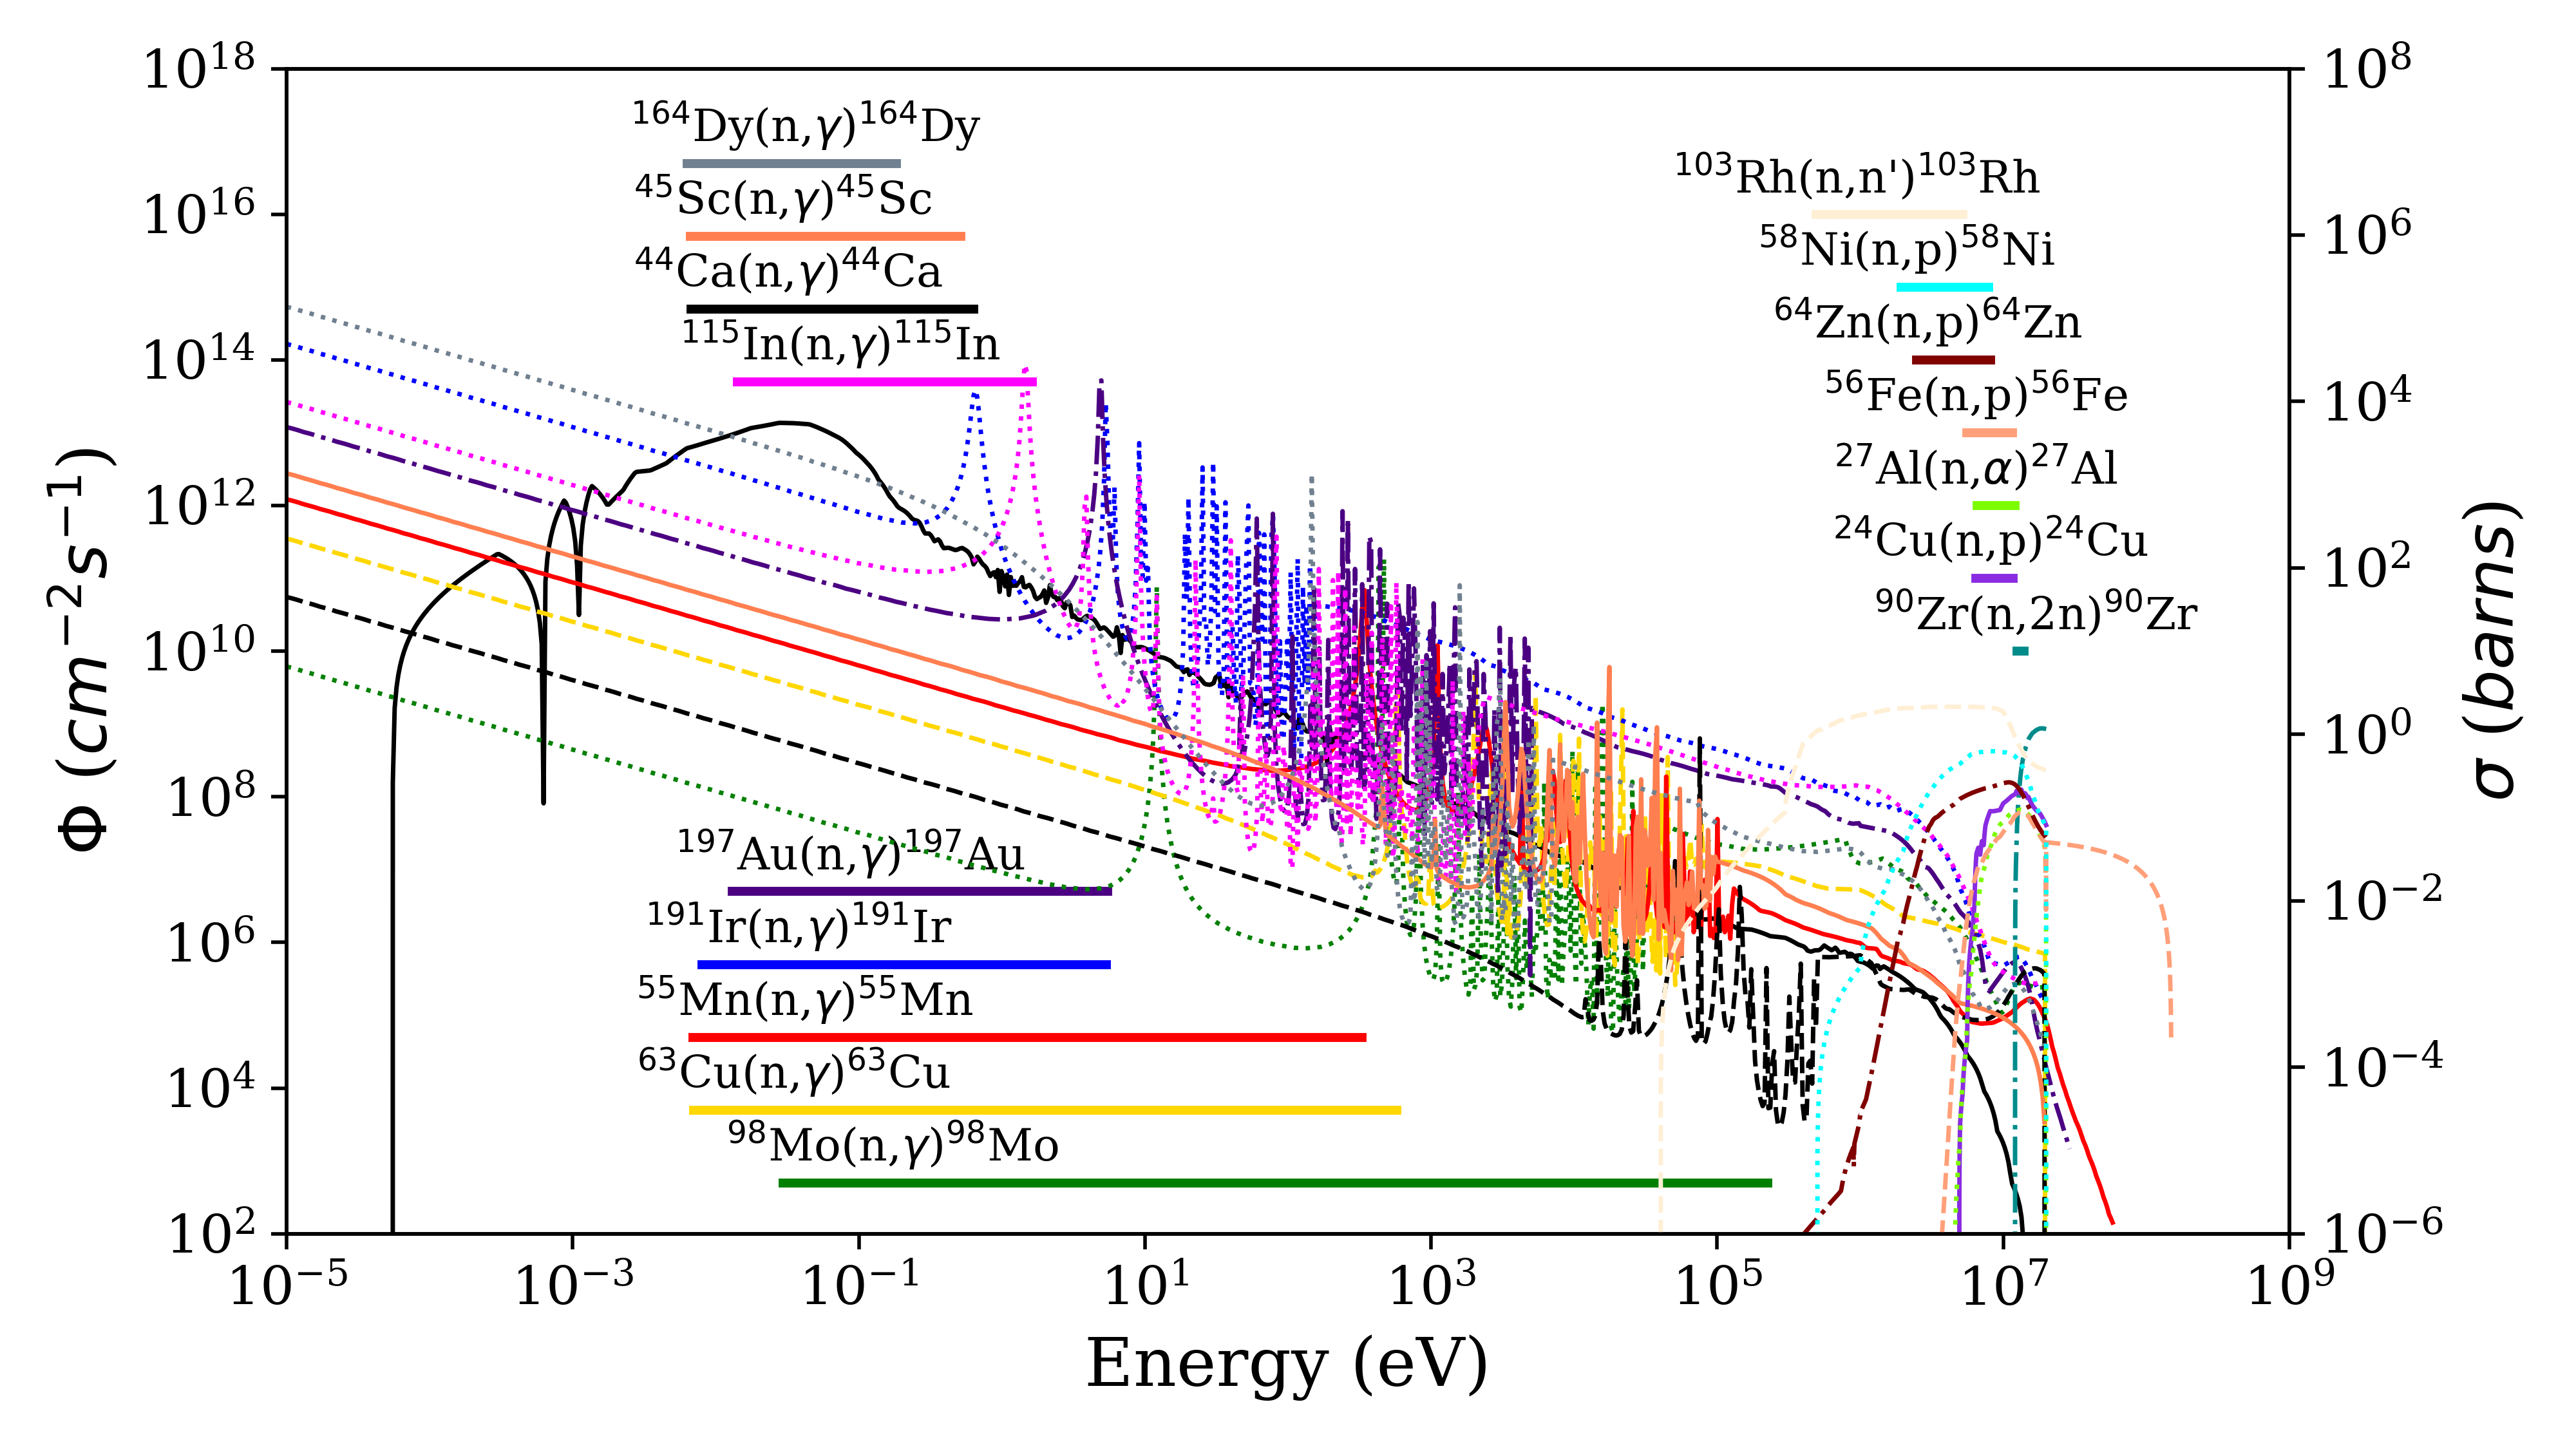
\includegraphics[width=1.0\textwidth]{plot/amalgamated}
   \label{fig:amalgamated}
\end{figure}



% full reaction table
\begin{table*}[h]
\centering
\begin{tabular}{ |c|c|c|c|c|c|c| }
 \hline
 Reaction & T$_{1/2}$ & ROI (eV) & Important Gammas (keV) \\
 \hline
 $^{115}$In(n,$\gamma$)$^{116}$In & 54 m & 7.0021e-03, 1.6130e+00 & 417, 819, 1090, 1293, 1508, 2111 \\
 \hline
  $^{115}$In(n,$\gamma$)$^{116}$In Cd & 54 m & 1.1955e+00, 1.9916e+00 & 417, 819, 1090, 1293, 1508, 2111 \\
 \hline
 $^{197}$Au(n,$\gamma$)$^{198}$Au & 2.7 d & 6.7266e-03, 5.2684e+00 & 412, 676, 1088 \\
 \hline
 $^{197}$Au(n,$\gamma$)$^{198}$Au Cd & 2.7 d & 4.0752e+00, 7.1730e+00 & 412, 676, 1088 \\
 \hline
 $^{103}$Rh(n,n')$^{103m}$Rh & 56.12 m & 4.4469e+05, 5.1947e+06 & 40 \\
 \hline
 $^{27}$Al(n,$\alpha$)$^{24}$Na & 15.03 h & 6.4564e+06, 1.1695e+07 & 1369, 2754 \\
 \hline
\end{tabular}
\end{table*}

\newpage

\newpage

\section*{ Indium }

Power Level: 1.0 kW(th) \\
Time at Power: 60 s \\
Wait Time: 400 s \\
Total Activity at Removal: 1.79e+02 $\mu Ci$

\begin{table*}[h]
\centering
\begin{tabular}{ |c|c|c|c|c|c|c| }
 \hline
 Position & Mass $mg$ & Start Counting $s$ & Counting Time $s$ & Counting Activity $\mu Ci$ \\
 \hline 
 1 & 1.7 & 460 & 300 & 4.51e+01\\ 
\hline
 2 & 1.5 & 760 & 300 & 3.73e+01\\ 
\hline
 3 & 1.4 & 1060 & 300 & 3.27e+01\\ 
\hline
 4 & 1.6 & 1360 & 300 & 3.50e+01\\ 
\hline
\end{tabular}
\end{table*}

\begin{figure}[!ht]
   \centering
   \subfloat[][Position \#1]{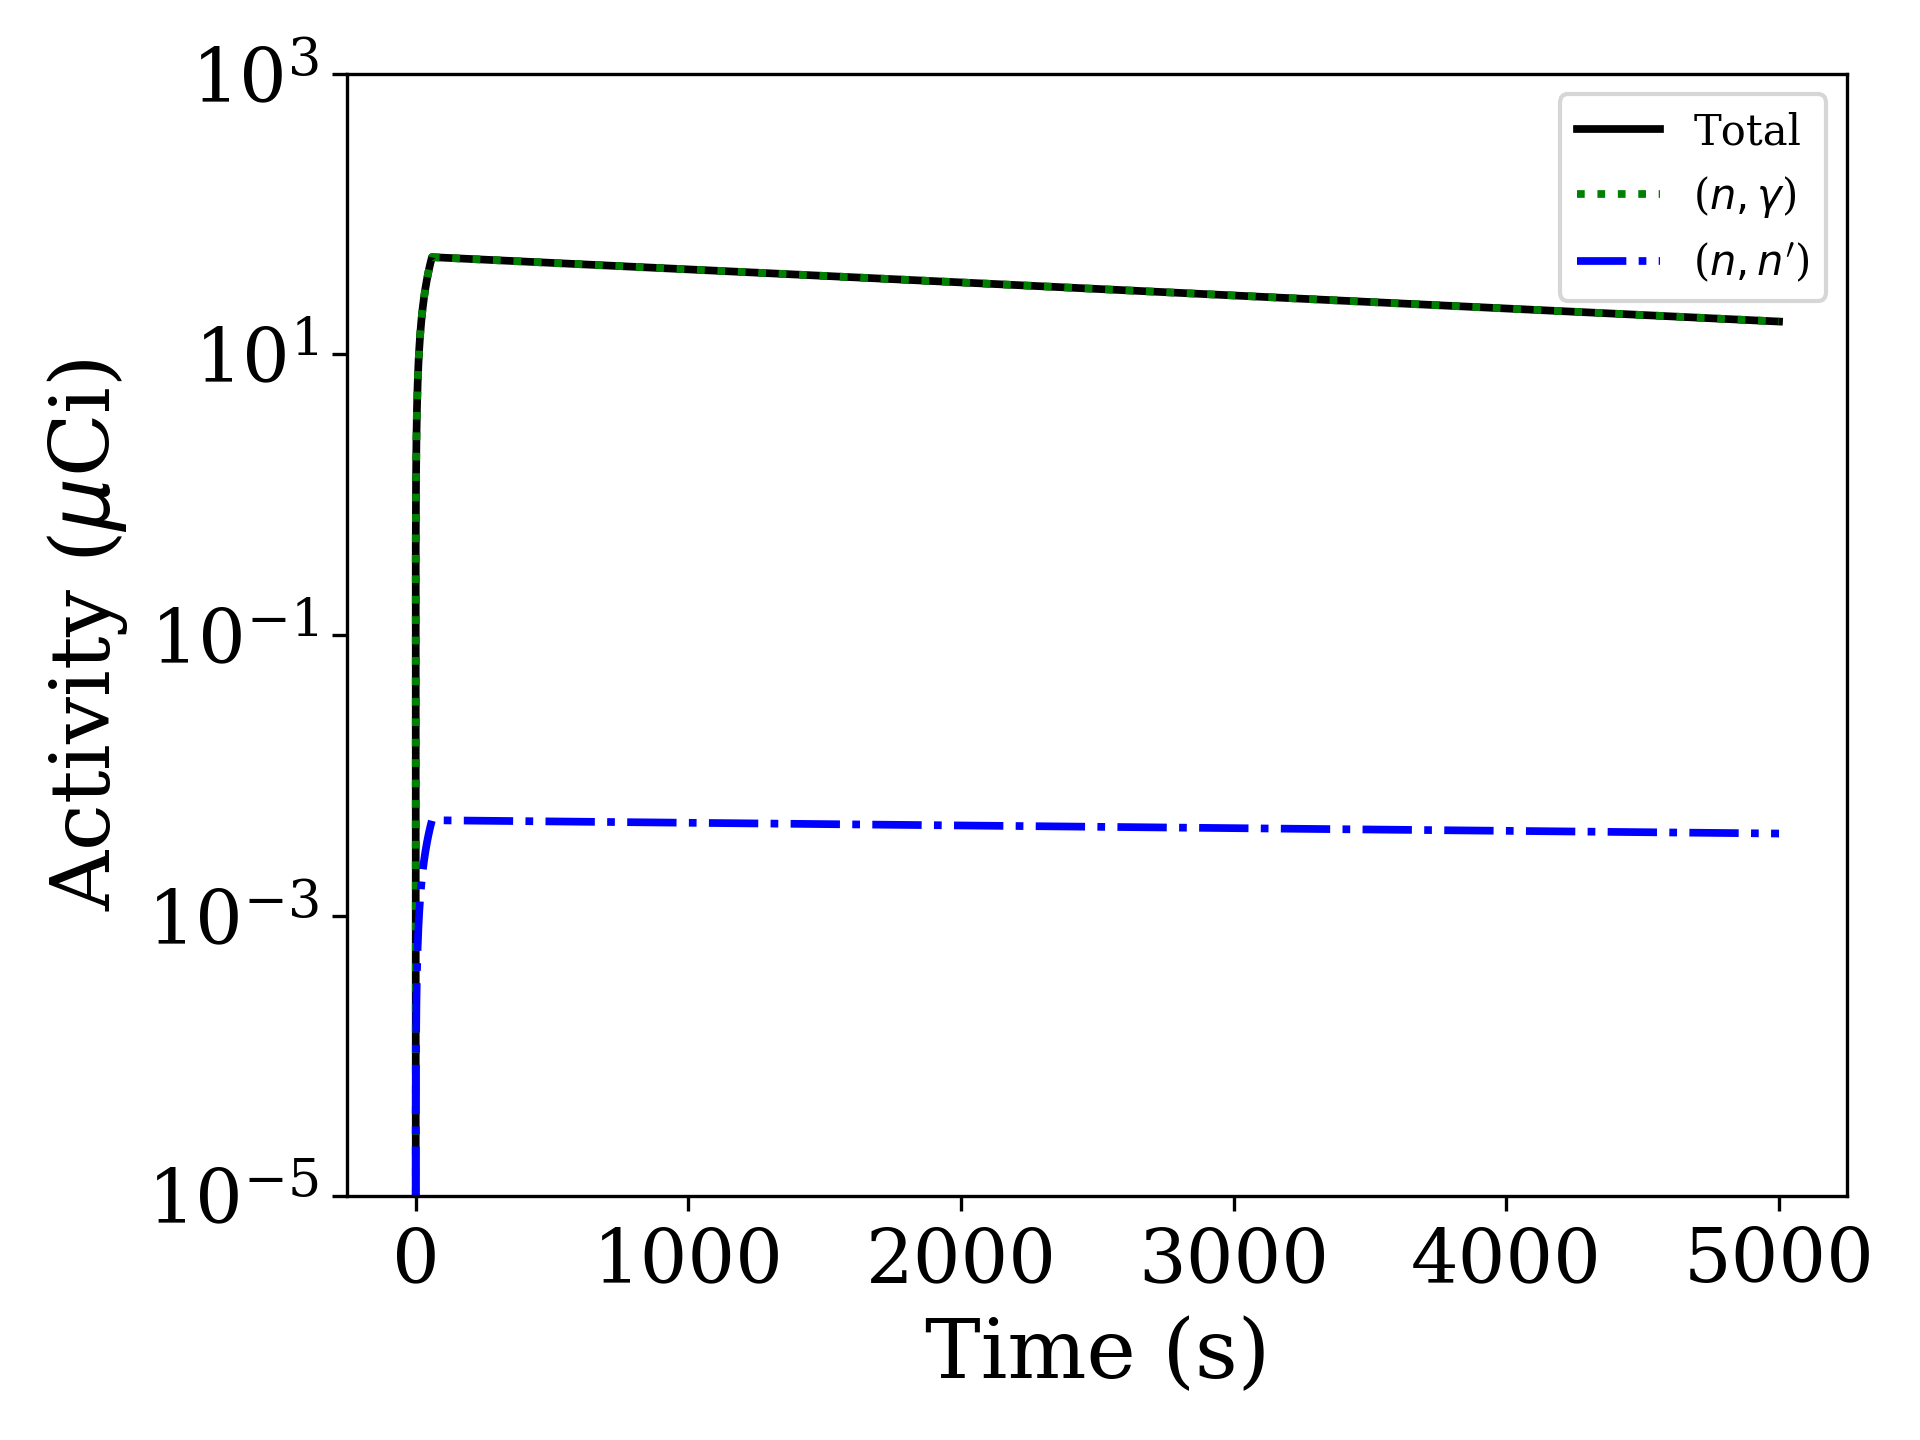
\includegraphics[width=.4\textwidth]{source/plot/in1_activity}}\quad
   \subfloat[][ ($n,\gamma$) Reaction Rate]{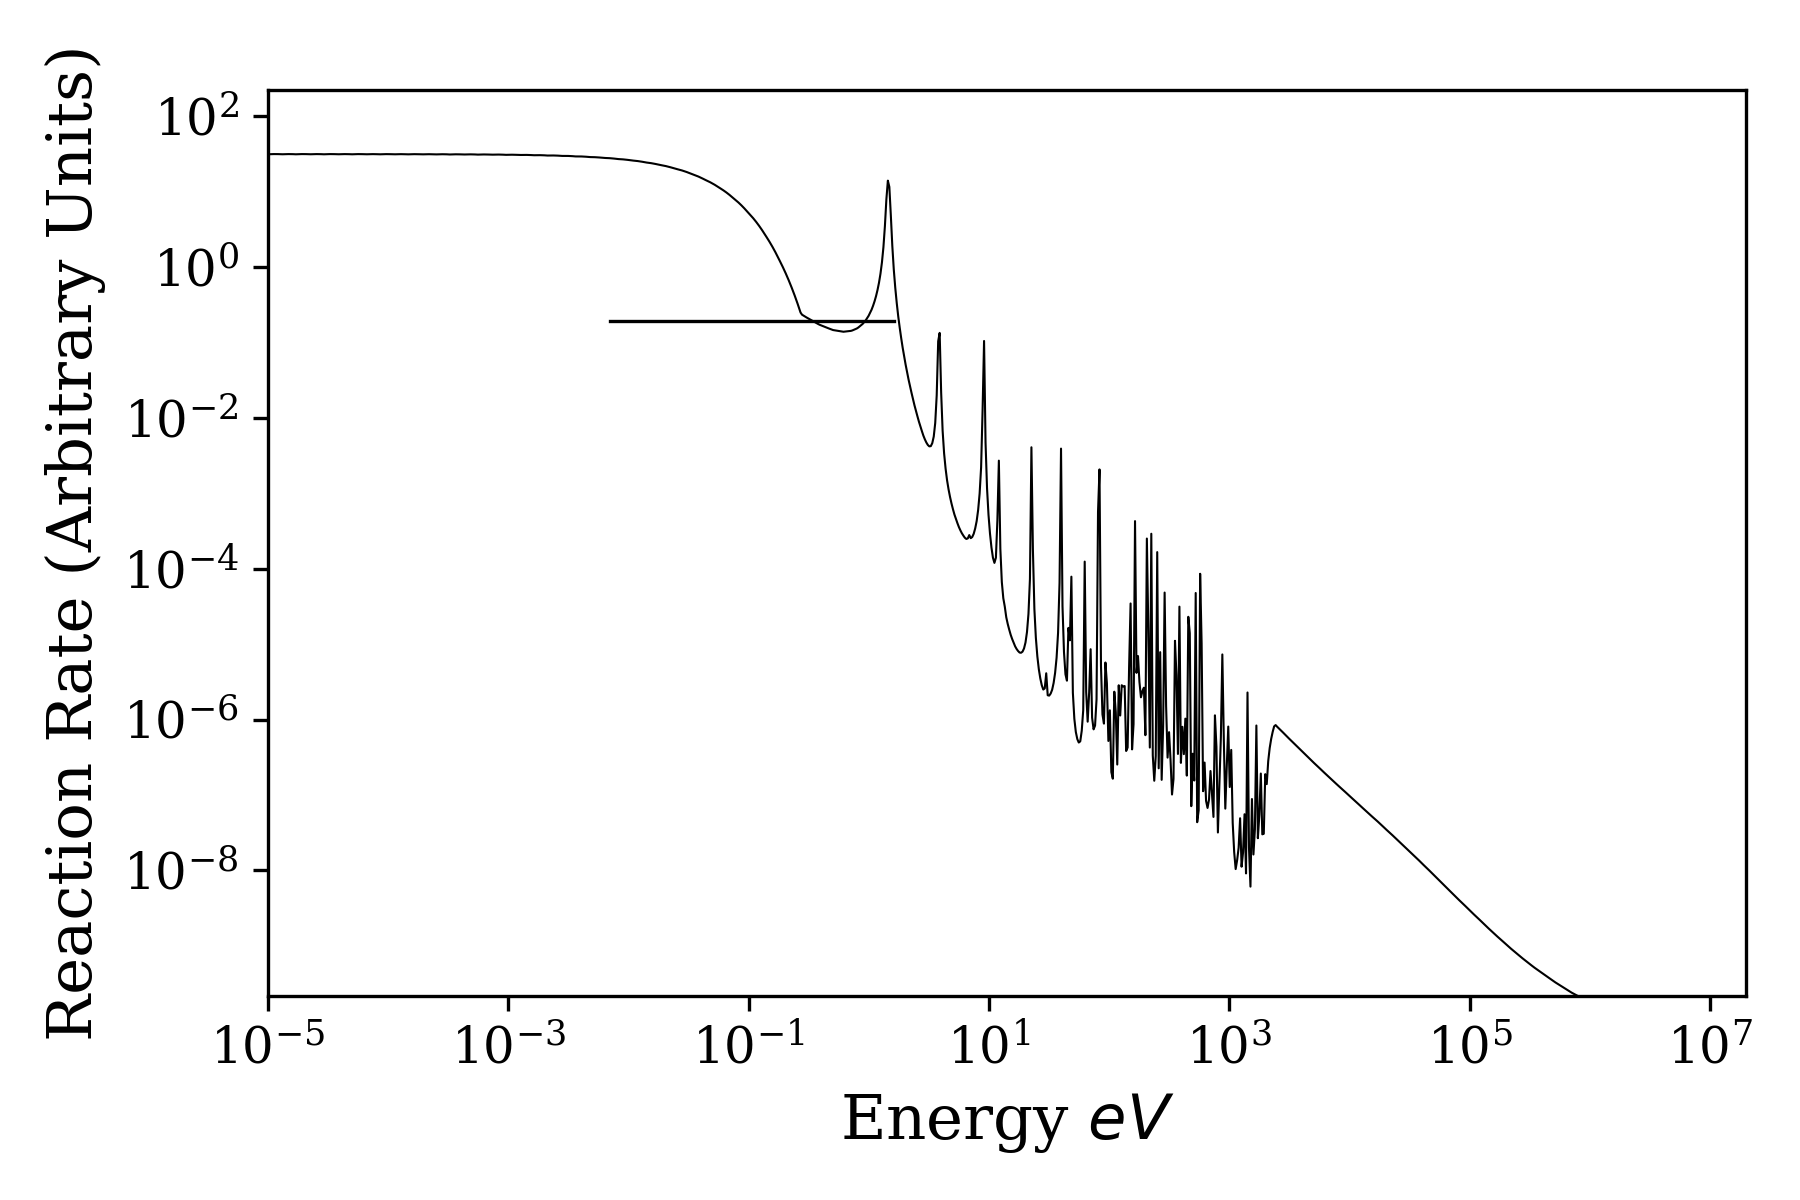
\includegraphics[width=.4\textwidth]{source/plot/in_n,gamma}}\\ 
   \subfloat[][ ($n,n'$) Reaction Rate]{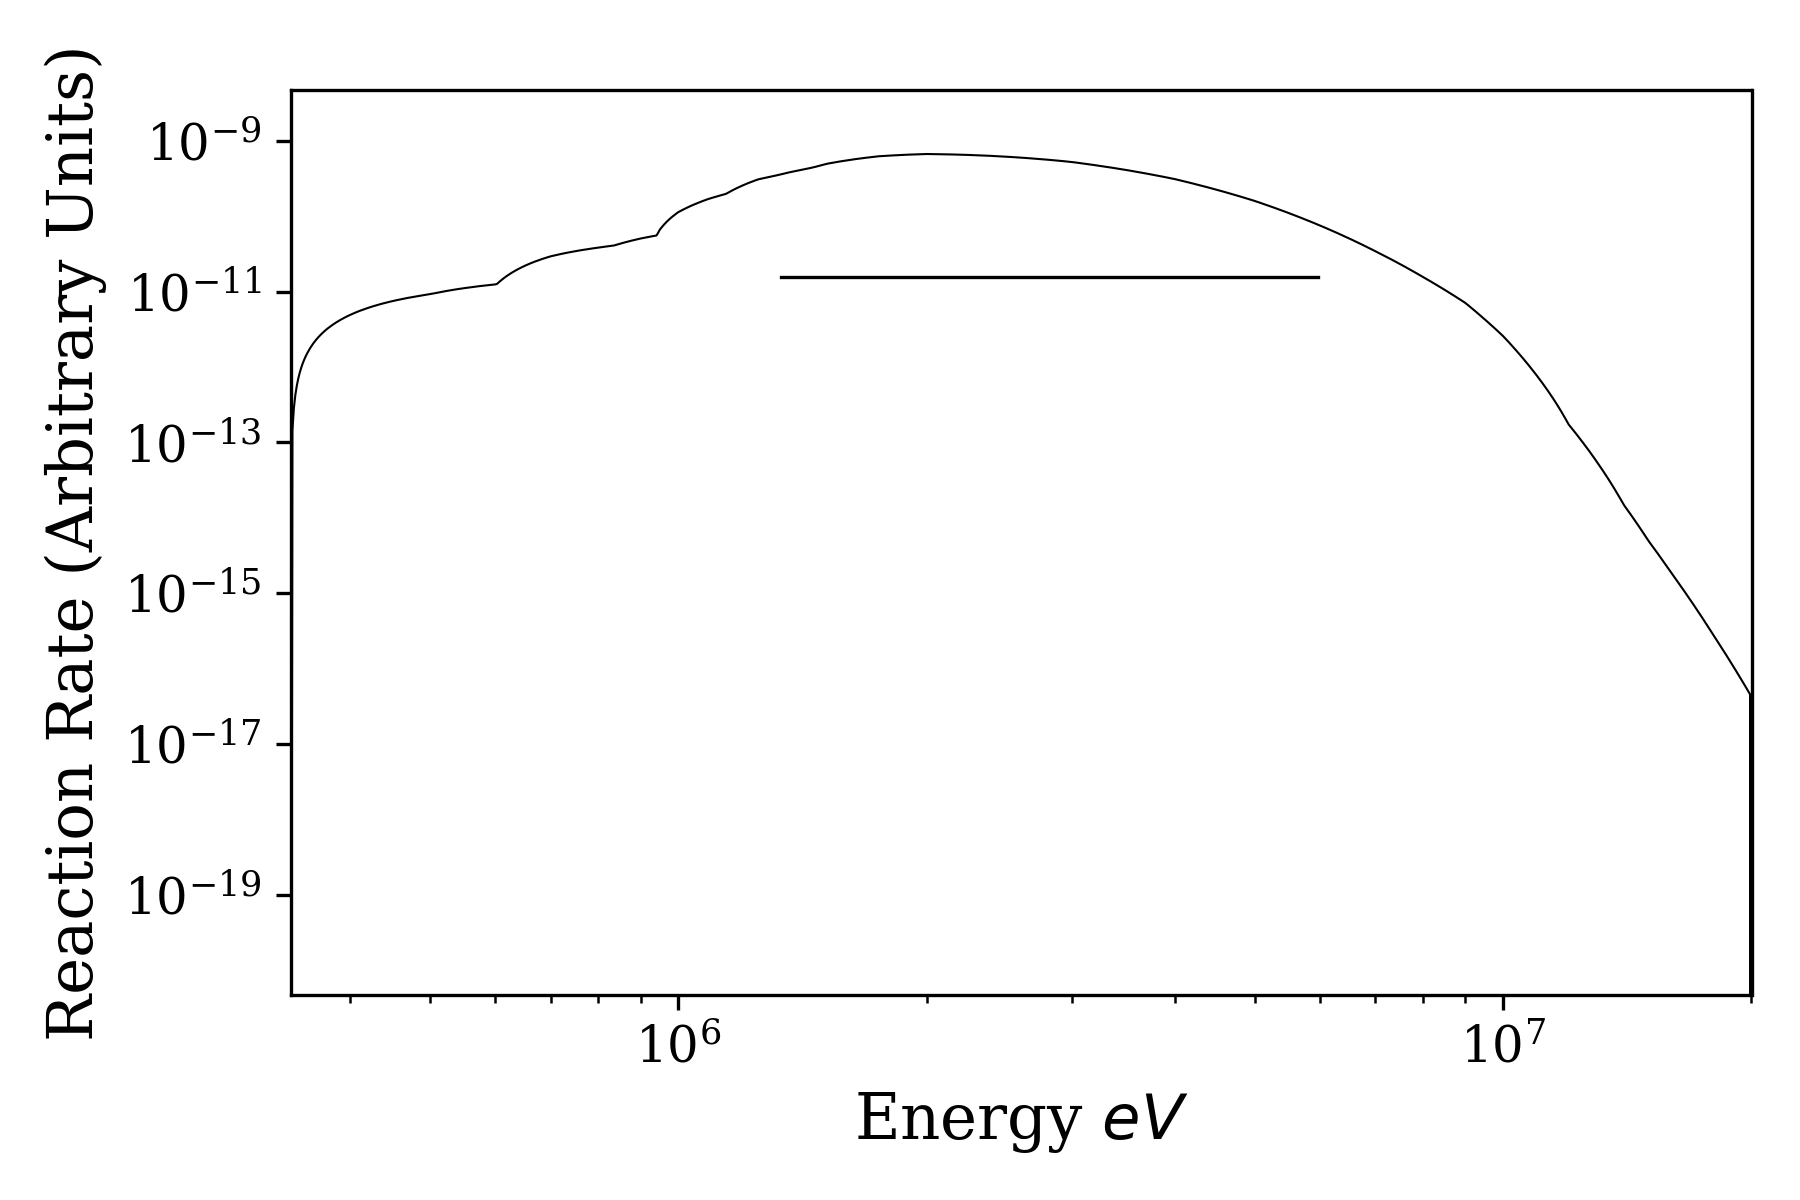
\includegraphics[width=.4\textwidth]{source/plot/in_n,inelastic}}\quad 

\end{figure}

\begin{table*}[h]
\centering
\begin{tabular}{ |c|c|c|c|c|c|c| }
 \hline
 Reaction & T$_{1/2}$ & ROI (eV) & Important Gammas (keV) \\
 \hline 
 ($n,\gamma$) & 54.0 m & 7.00e-03, 1.61e+00 & 138(0.03), 417(0.36), 819(0.17), 1090(0.53), 1293(0.8), 1508(0.11), 2111(0.2) \\ 
\hline
 ($n,n'$) &  4.4 h & 1.33e+06, 5.96e+06 & 335(0.5) \\ 
\hline
\end{tabular}
\end{table*}

\newpage

\section*{ Indium  (Cd) }

Power Level: 100.0 kW(th) \\
Time at Power: 60 s \\
Wait Time: 3600 s \\
Total Activity at Removal: 8.83e+03 $\mu Ci$

\begin{table*}[h]
\centering
\begin{tabular}{ |c|c|c|c|c|c|c| }
 \hline
 Position & Mass $mg$ & Start Counting $s$ & Counting Time $s$ & Counting Activity $\mu Ci$ \\
 \hline 
 1 & 1.7 & 3660 & 300 & 1.12e+03\\ 
\hline
 2 & 1.5 & 3960 & 300 & 9.30e+02\\ 
\hline
 3 & 1.4 & 4260 & 300 & 8.14e+02\\ 
\hline
 4 & 1.6 & 4560 & 300 & 8.73e+02\\ 
\hline
\end{tabular}
\end{table*}

\begin{figure}[!ht]
   \centering
   \subfloat[][Position \#1]{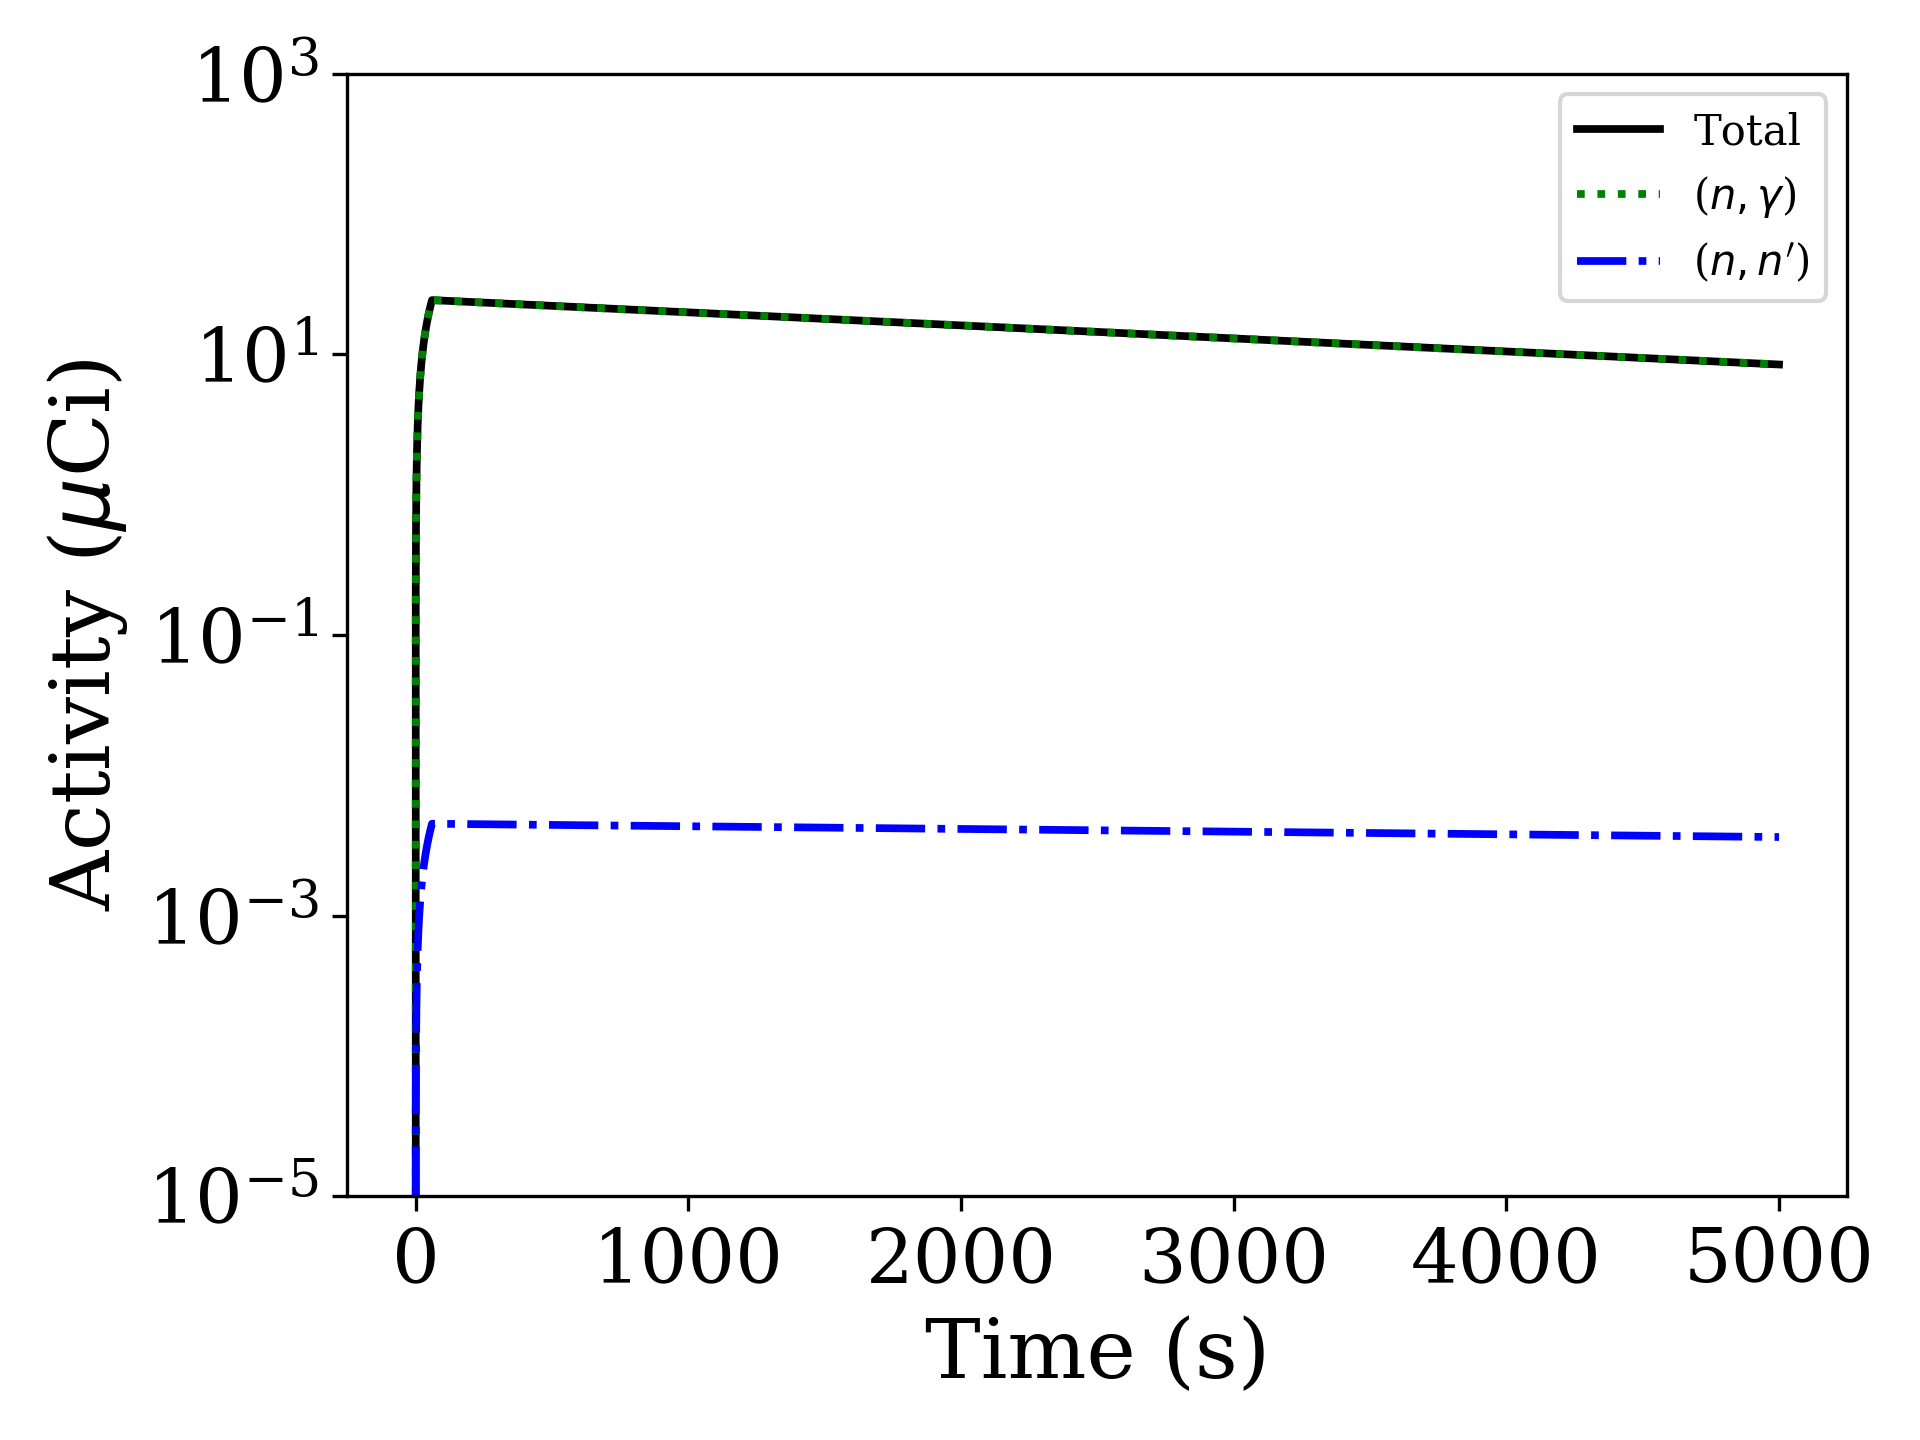
\includegraphics[width=.4\textwidth]{source/plot/in1cd_activity}}\quad
   \subfloat[][ ($n,\gamma$) Reaction Rate]{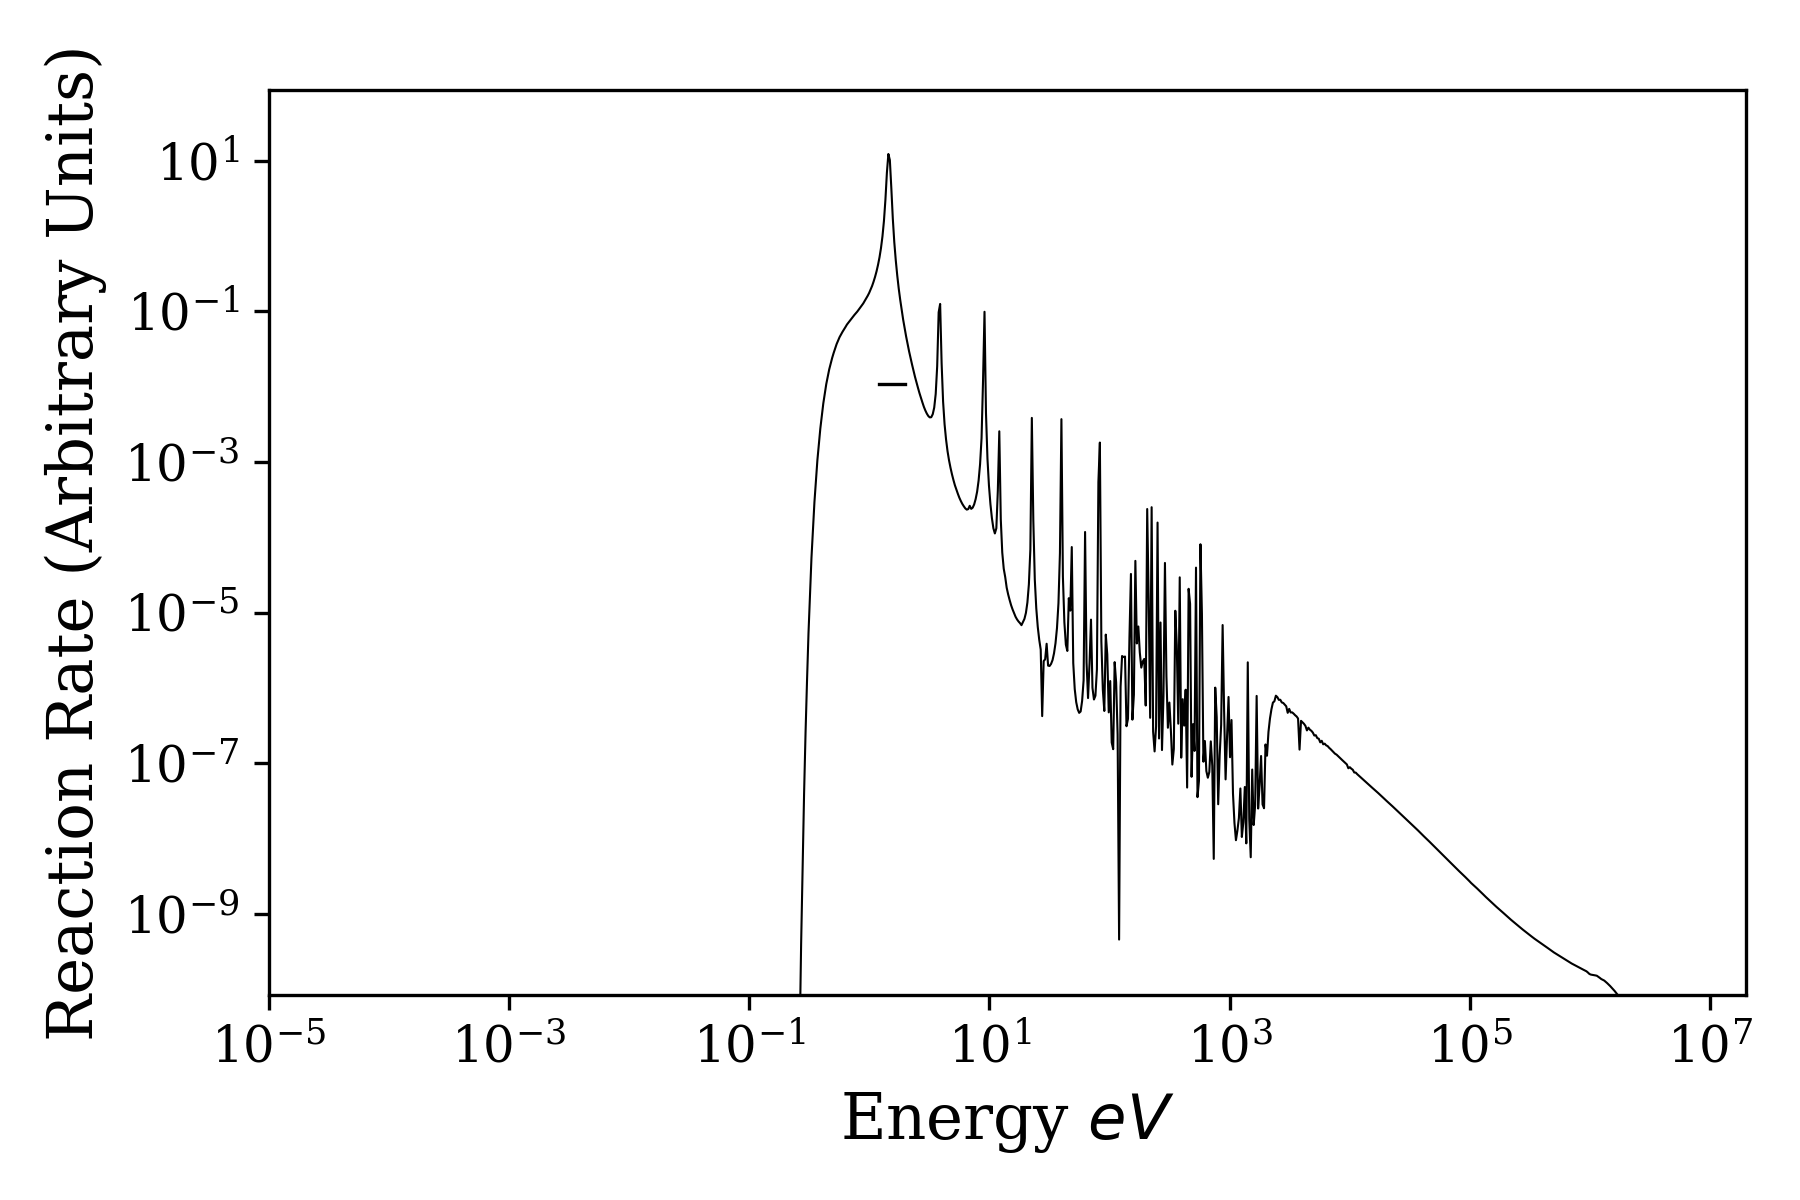
\includegraphics[width=.4\textwidth]{source/plot/in_n,gamma_cd}}\\ 
   \subfloat[][ ($n,n'$) Reaction Rate]{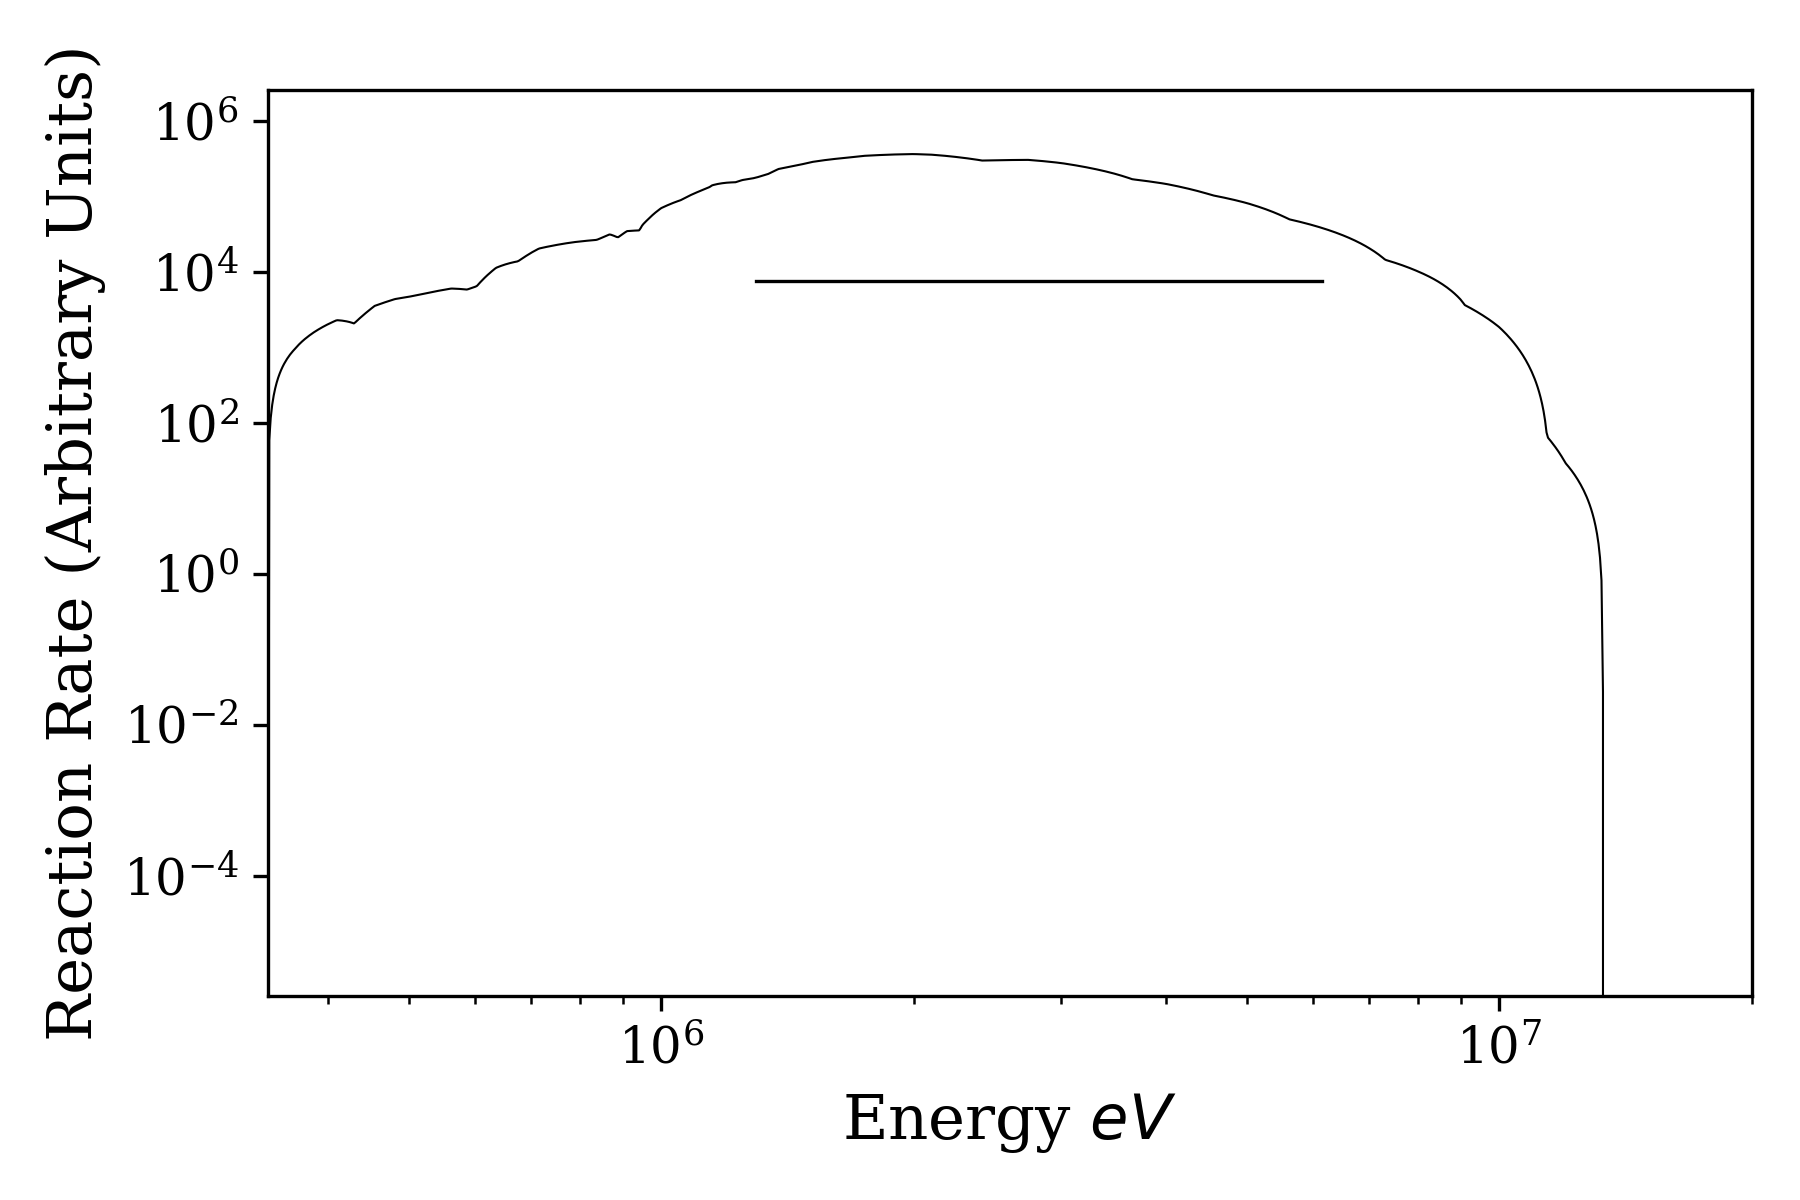
\includegraphics[width=.4\textwidth]{source/plot/in_n,inelastic_cd}}\quad 

\end{figure}

\begin{table*}[h]
\centering
\begin{tabular}{ |c|c|c|c|c|c|c| }
 \hline
 Reaction & T$_{1/2}$ & ROI (eV) & Important Gammas (keV) \\
 \hline 
 ($n,\gamma$) & 54.0 m & 1.20e+00, 1.99e+00 & 138(0.03), 417(0.36), 819(0.17), 1090(0.53), 1293(0.8), 1508(0.11), 2111(0.2) \\ 
\hline
 ($n,n'$) &  4.4 h & 1.34e+06, 5.97e+06 & 335(0.5) \\ 
\hline
\end{tabular}
\end{table*}

\newpage

\section*{ Gold }

Power Level: 100 kW(th) \\
Time at Power: 60 s \\
Wait Time: 3600 s \\
Total Activity at Removal: 2.78e+03 $\mu Ci$

\begin{table*}[h]
\centering
\begin{tabular}{ |c|c|c|c|c|c|c| }
 \hline
 Position & Mass $mg$ & Start Counting $s$ & Counting Time $s$ & Counting Activity $\mu Ci$ \\
 \hline 
 1 & 5.0 & 3660 & 300 & 5.60e+01\\ 
\hline
 2 & 4.35 & 3960 & 300 & 4.87e+01\\ 
\hline
 3 & 4.3 & 4260 & 300 & 4.81e+01\\ 
\hline
 4 & 4.37 & 4560 & 300 & 4.88e+01\\ 
\hline
\end{tabular}
\end{table*}

\begin{figure}[!ht]
   \centering
   \subfloat[][Position \#1]{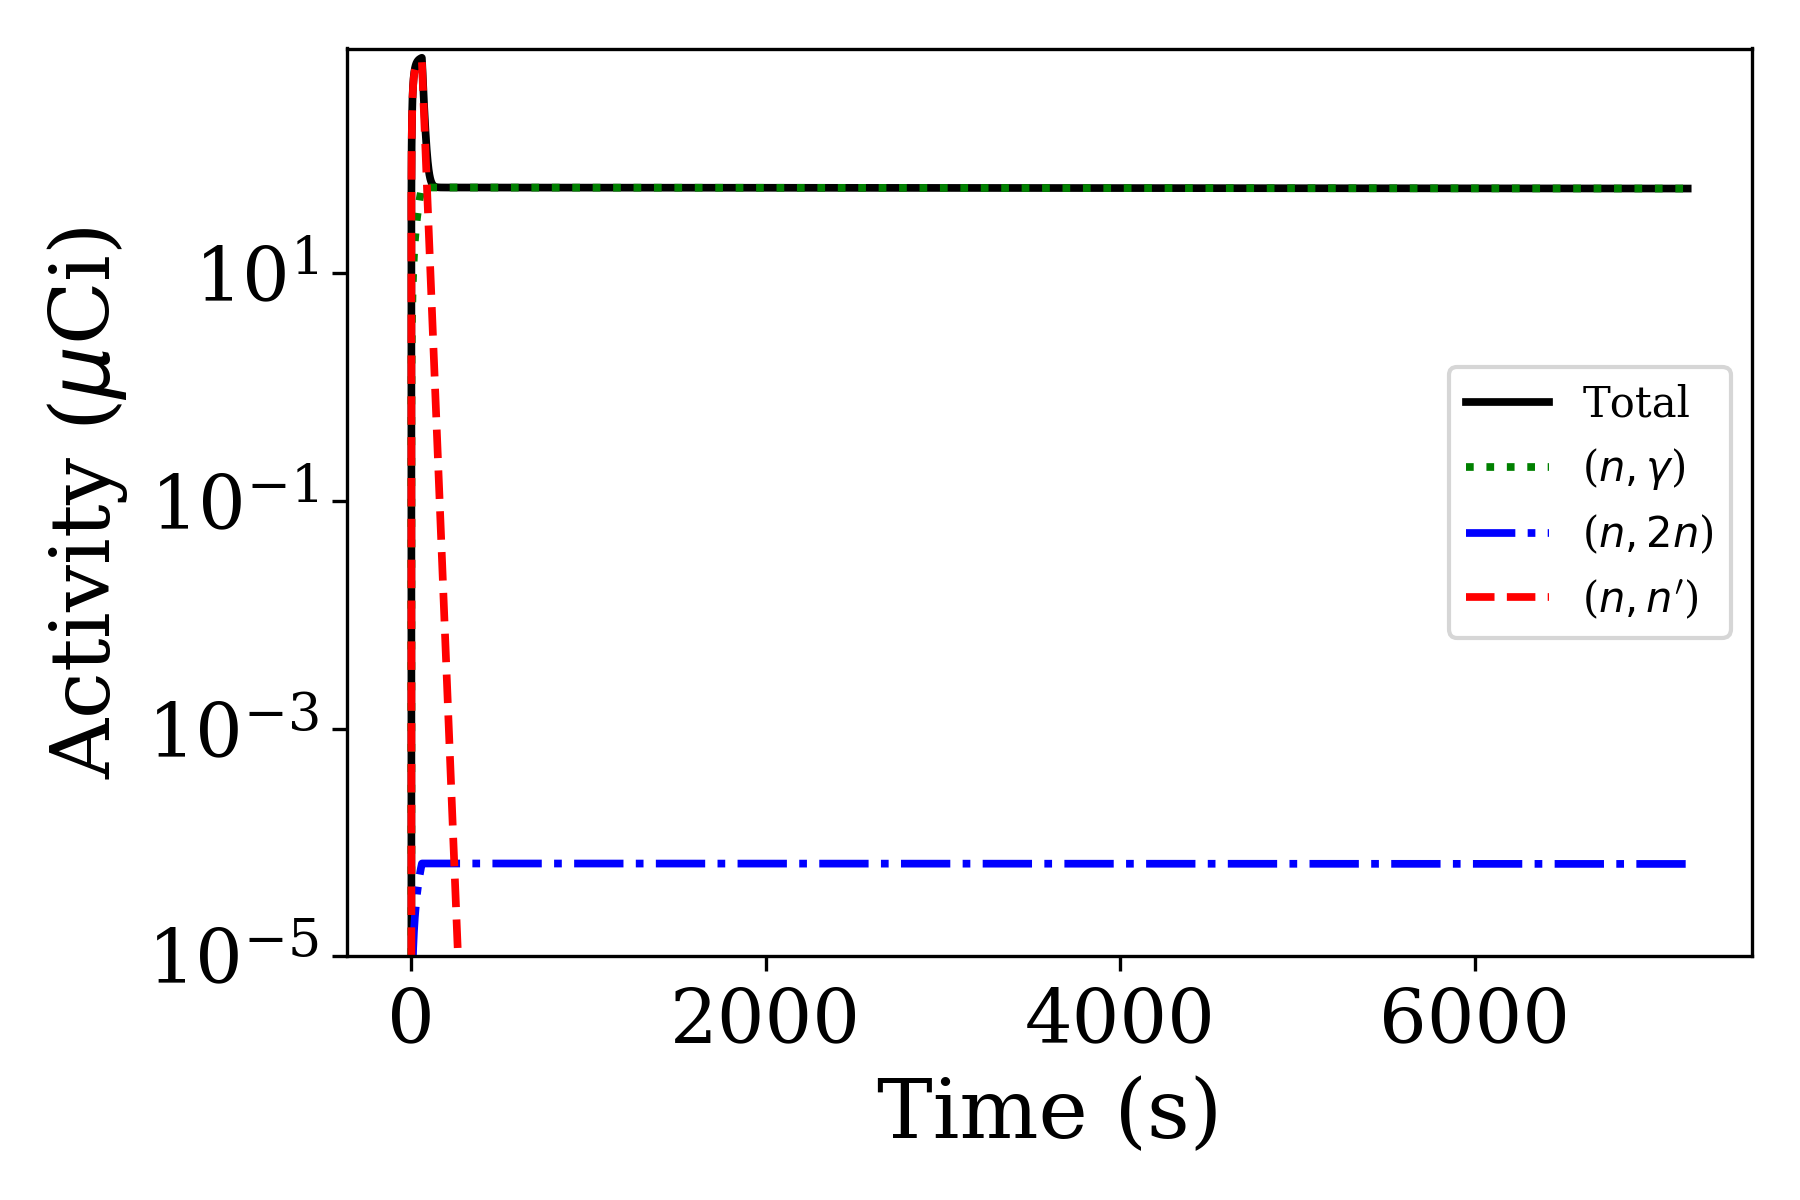
\includegraphics[width=.4\textwidth]{source/plot/au1_activity}}\quad
   \subfloat[][ ($n,\gamma$) Reaction Rate]{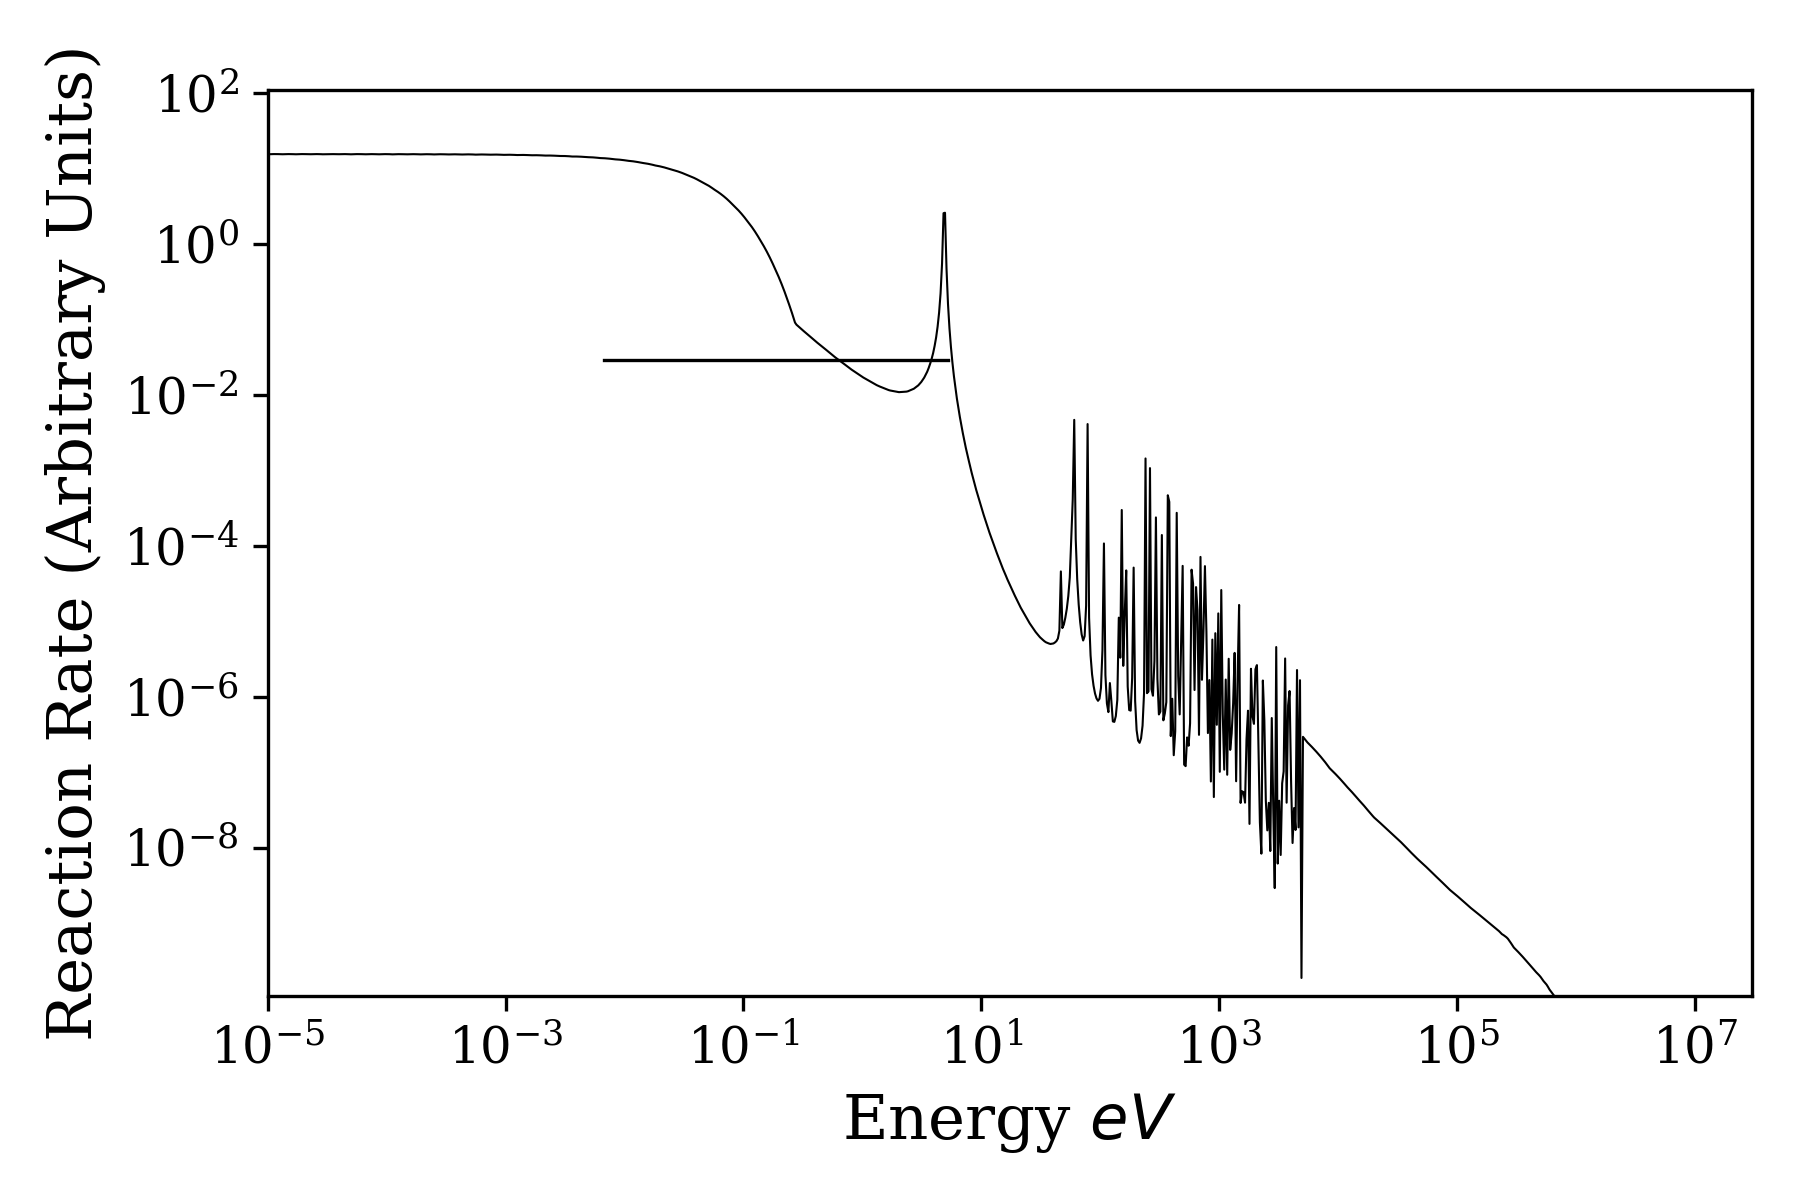
\includegraphics[width=.4\textwidth]{source/plot/au_n,gamma}}\\ 
   \subfloat[][ ($n,2n$) Reaction Rate]{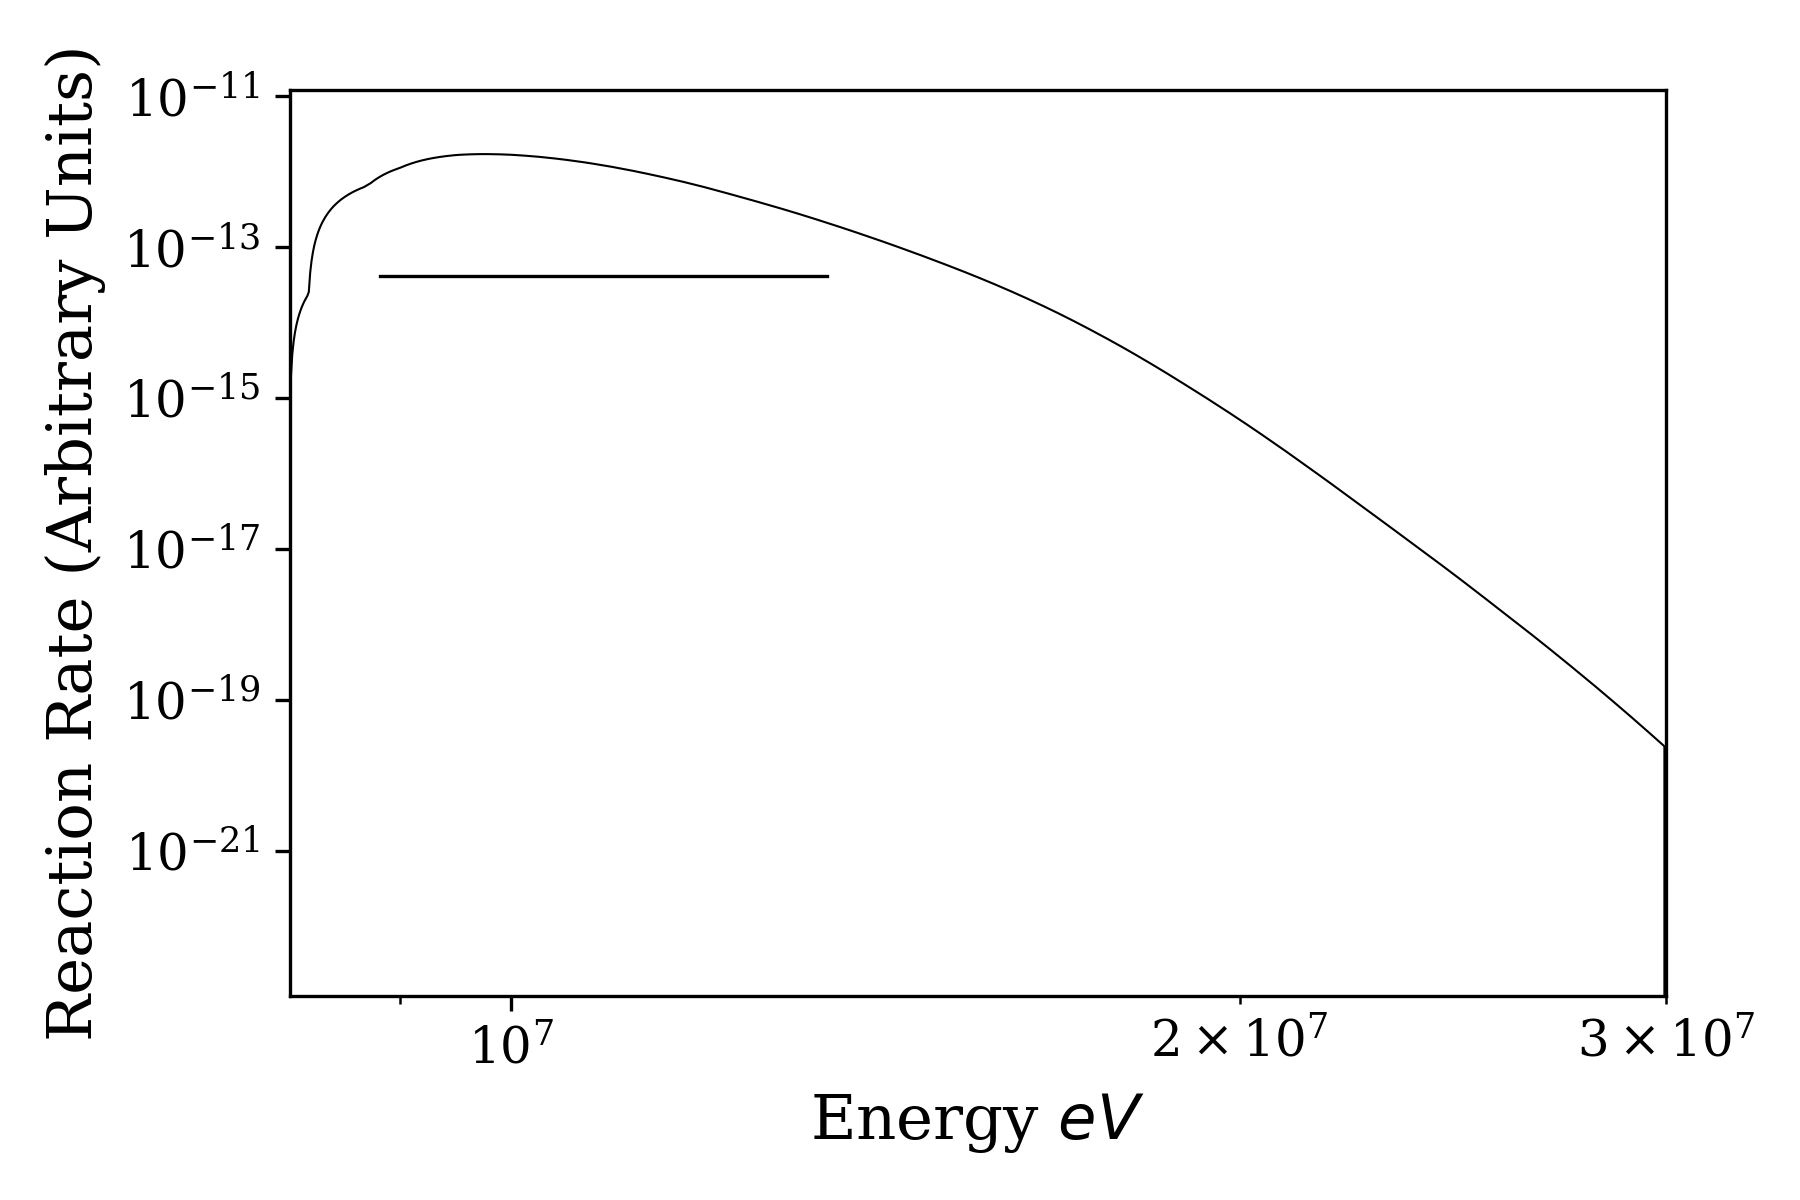
\includegraphics[width=.4\textwidth]{source/plot/au_n,2n}}\quad 
   \subfloat[][ ($n,n'$) Reaction Rate]{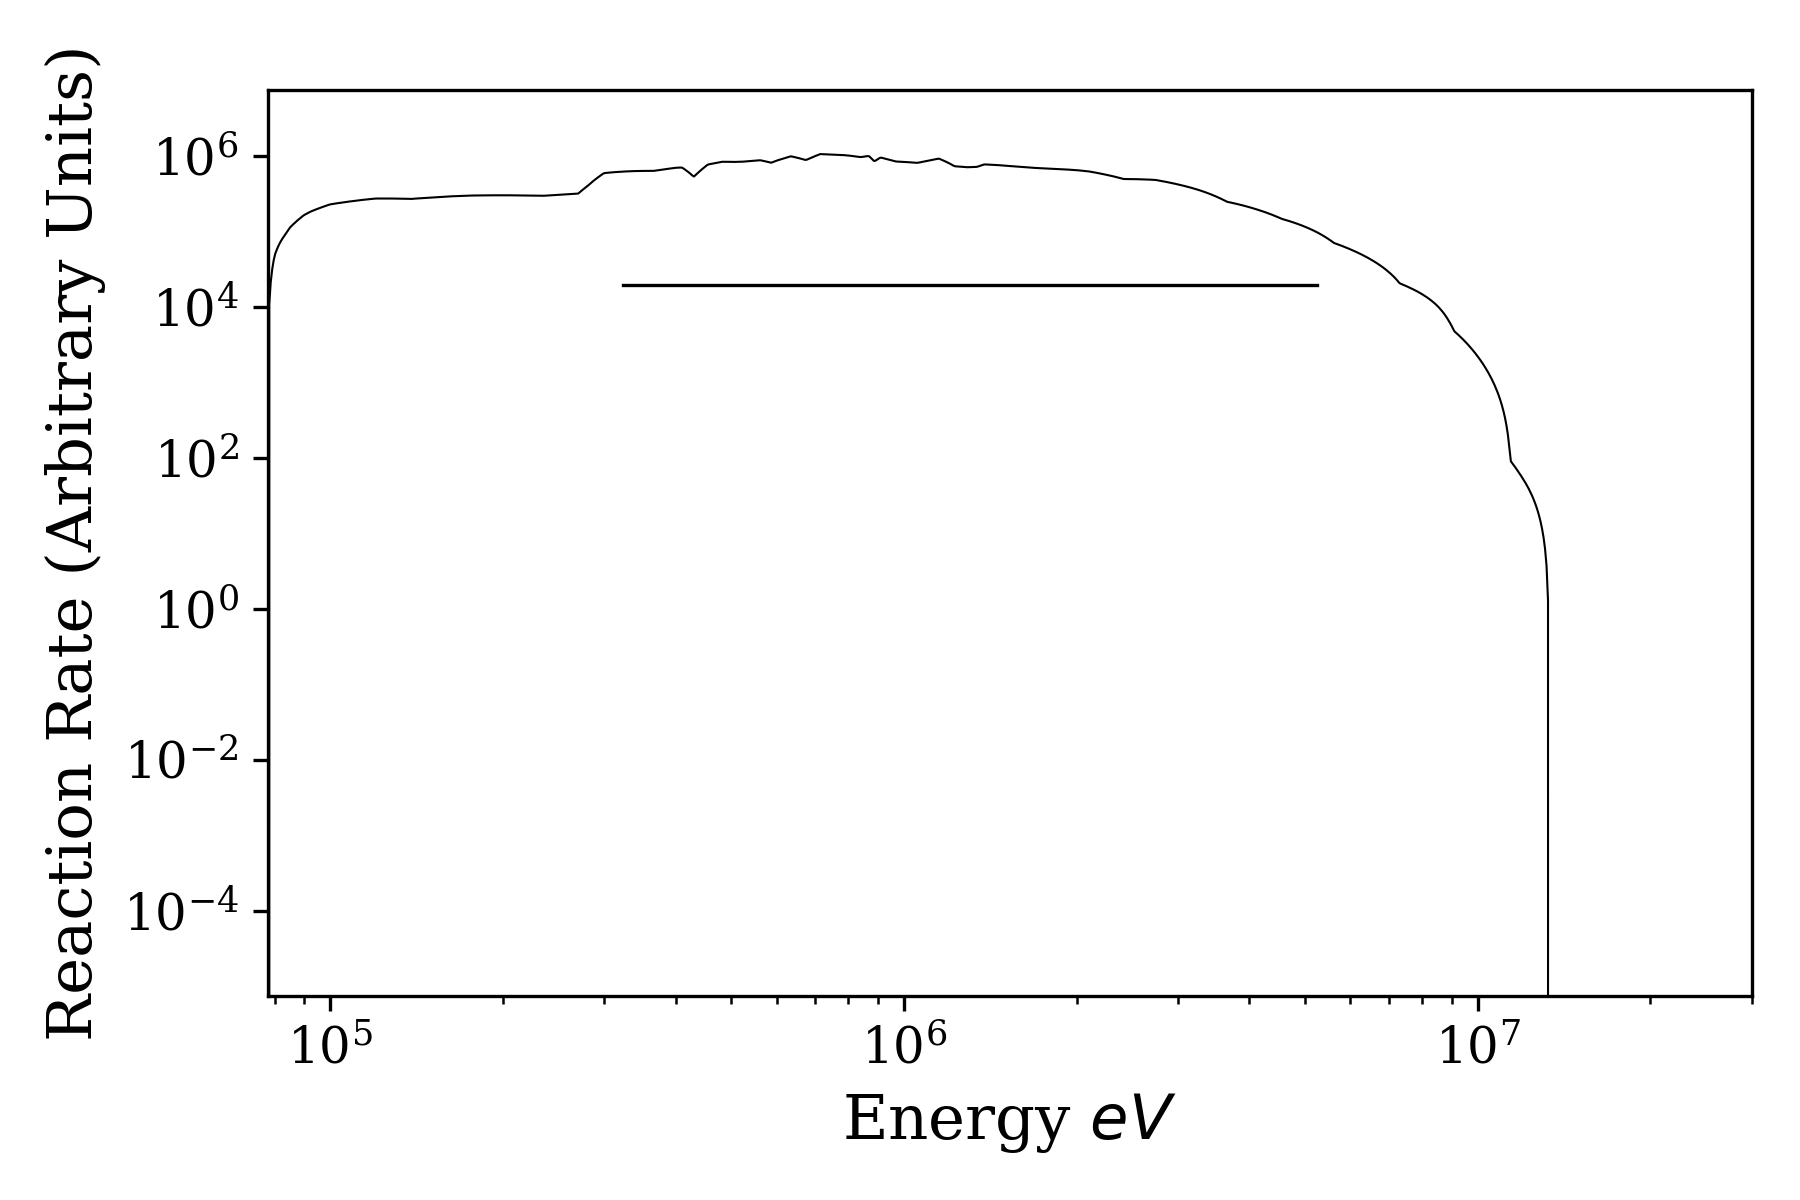
\includegraphics[width=.4\textwidth]{source/plot/au_n,inelastic}}\\ 

\end{figure}

\begin{table*}[h]
\centering
\begin{tabular}{ |c|c|c|c|c|c|c| }
 \hline
 Reaction & T$_{1/2}$ & ROI (eV) & Important Gammas (keV) \\
 \hline 
 ($n,\gamma$) &  2.7 d & 6.73e-03, 5.27e+00 & 412(0.95), 676(0.01), 1088(0.002) \\ 
\hline
 ($n,2n$) &  6.2 d & 8.83e+06, 1.35e+07 & 333(0.25), 356(0.94), 426(0.06), 1091(0.002) \\ 
\hline
 ($n,n'$) &  7.8 s & 3.24e+05, 5.25e+06 & 130(0.08), 279(0.75) \\ 
\hline
\end{tabular}
\end{table*}

\newpage

\section*{ Gold  (Cd) }

Power Level: 100 kW(th) \\
Time at Power: 45 s \\
Wait Time: 300 s \\
Total Activity at Removal: 2.49e+03 $\mu Ci$

\begin{table*}[h]
\centering
\begin{tabular}{ |c|c|c|c|c|c|c| }
 \hline
 Position & Mass $mg$ & Start Counting $s$ & Counting Time $s$ & Counting Activity $\mu Ci$ \\
 \hline 
 1 & 5.0 & 345 & 300 & 2.28e+01\\ 
\hline
 2 & 4.35 & 645 & 300 & 1.98e+01\\ 
\hline
 3 & 4.3 & 945 & 300 & 1.96e+01\\ 
\hline
 4 & 4.37 & 1245 & 300 & 1.99e+01\\ 
\hline
\end{tabular}
\end{table*}

\begin{figure}[!ht]
   \centering
   \subfloat[][Position \#1]{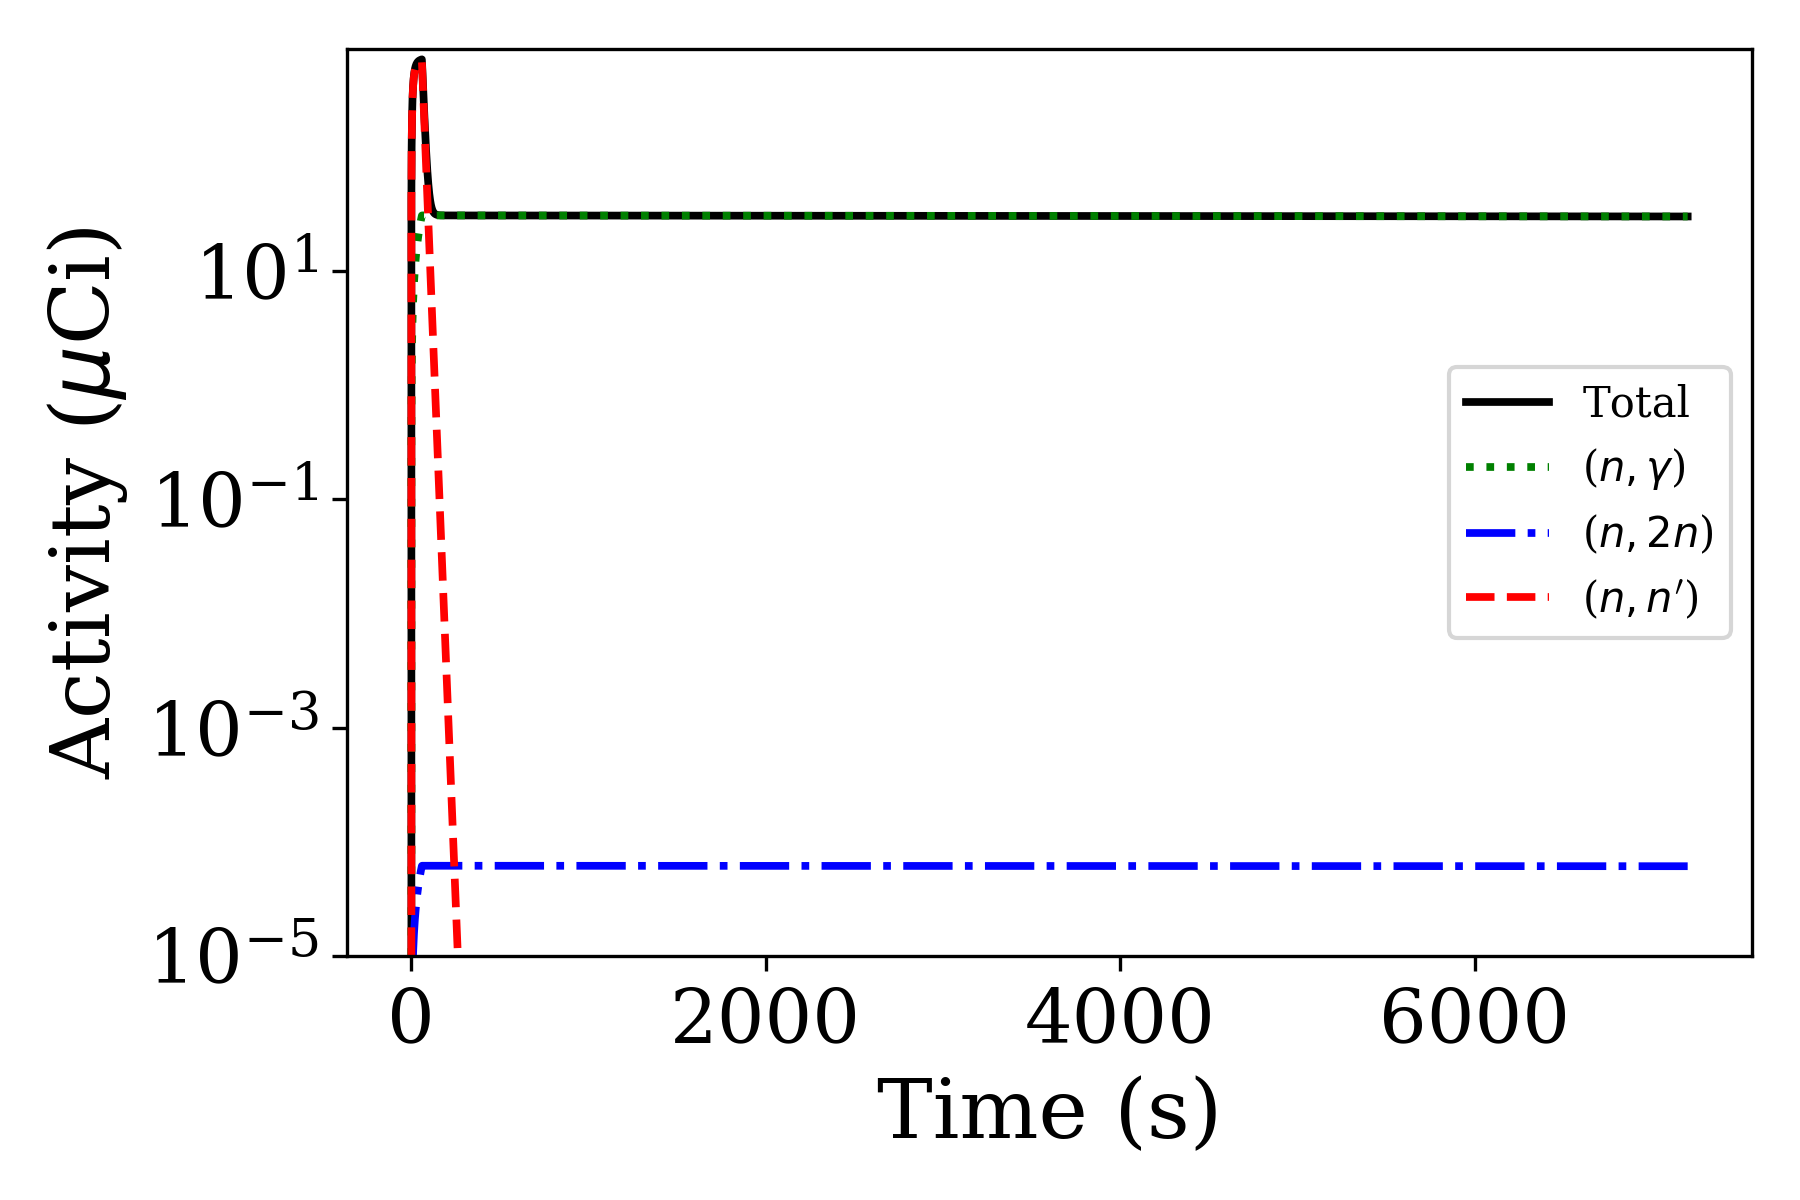
\includegraphics[width=.4\textwidth]{plot/au1cd_activity}}\quad
   \subfloat[][ ($n,\gamma$) Reaction Rate]{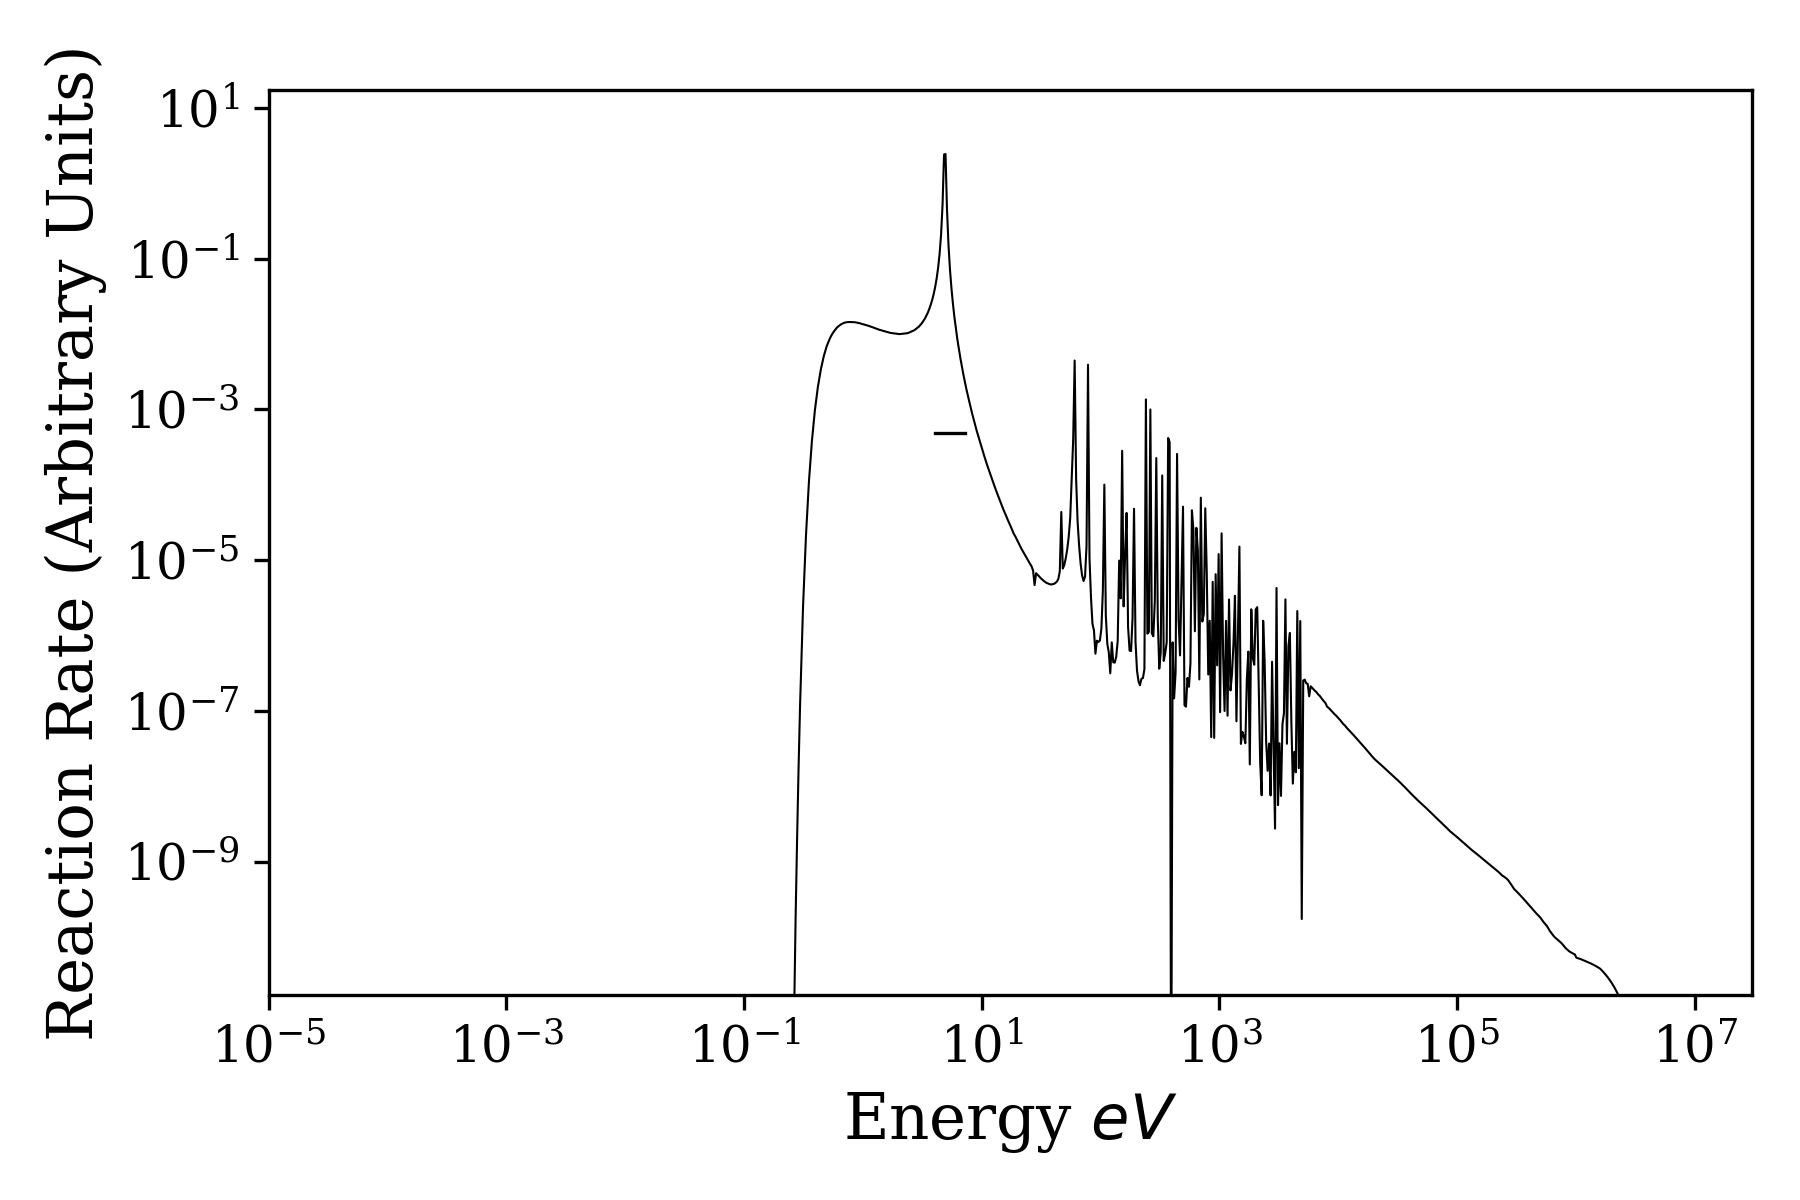
\includegraphics[width=.4\textwidth]{plot/au_n,gamma_cd}}\\ 
   \subfloat[][ ($n,2n$) Reaction Rate]{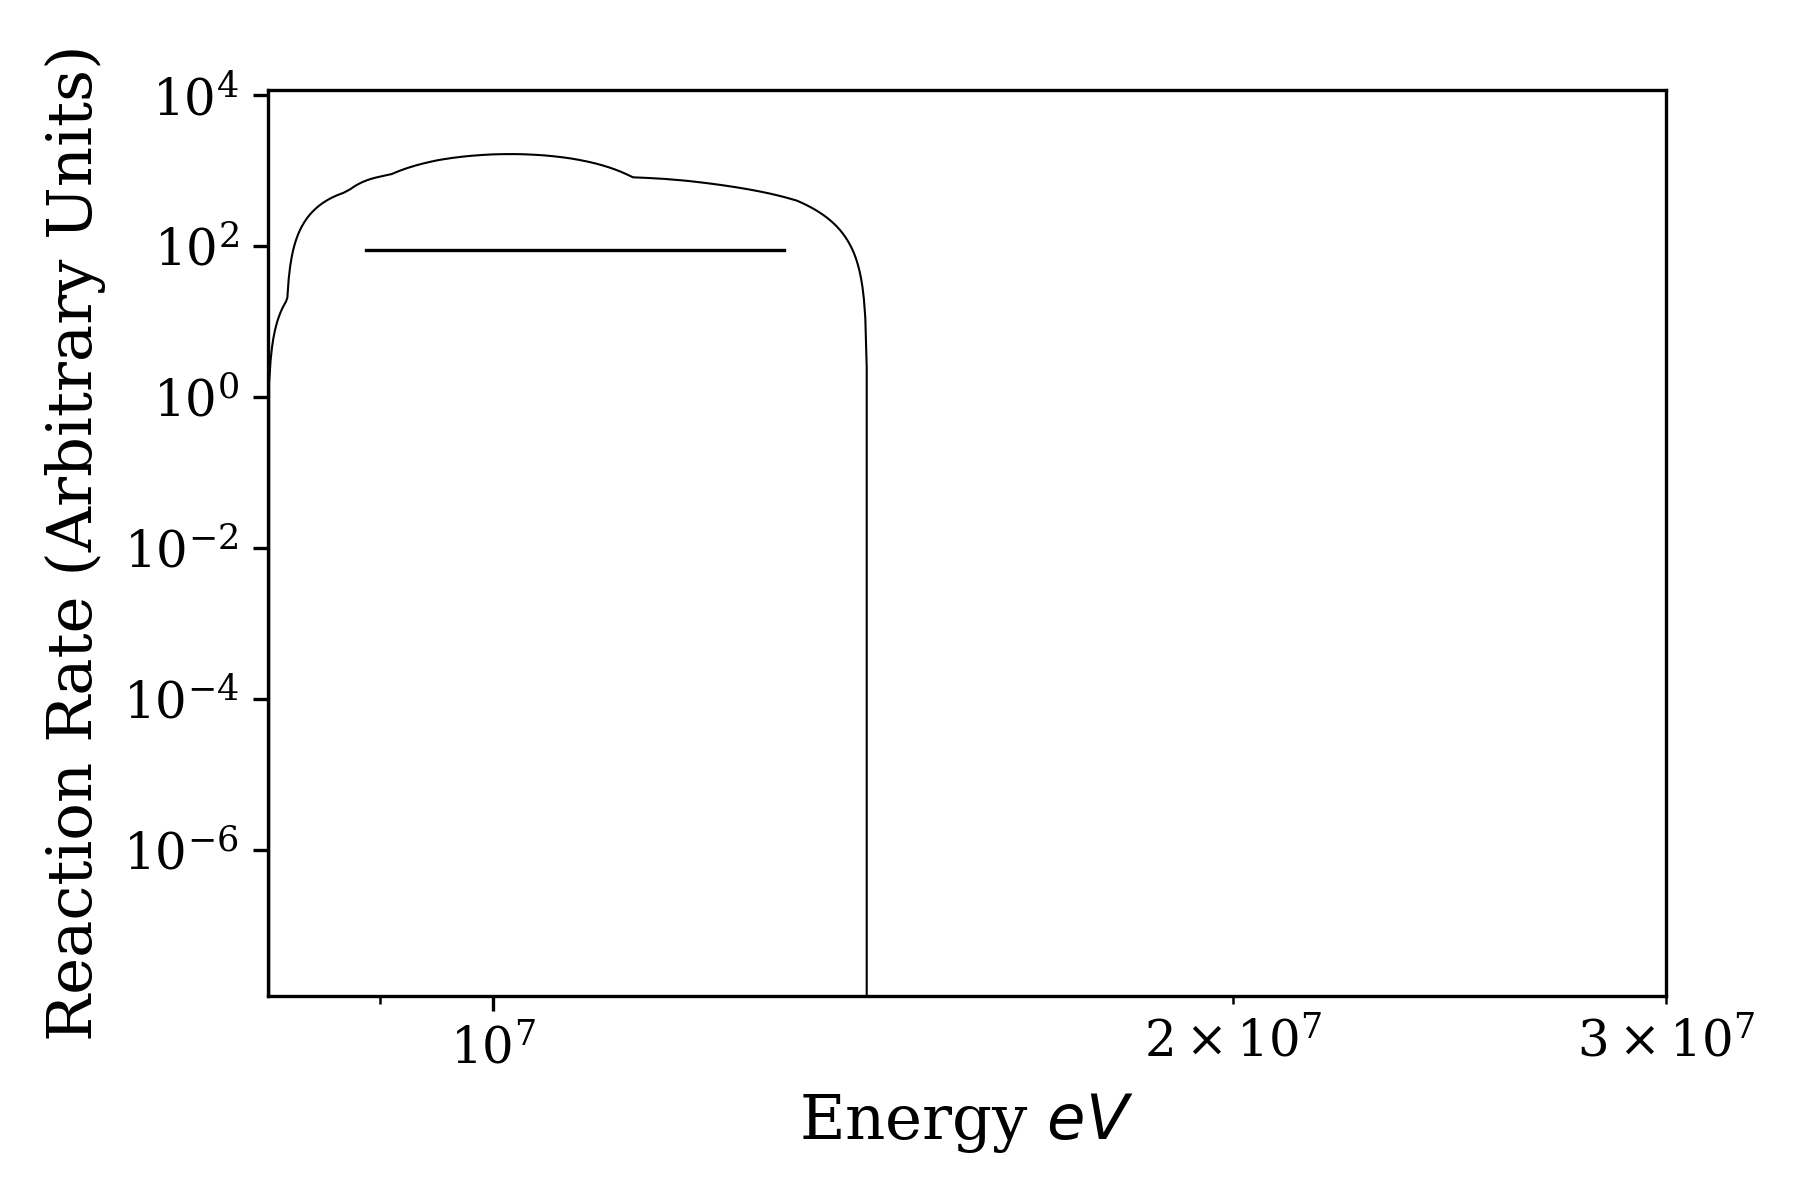
\includegraphics[width=.4\textwidth]{plot/au_n,2n_cd}}\quad 
   \subfloat[][ ($n,n'$) Reaction Rate]{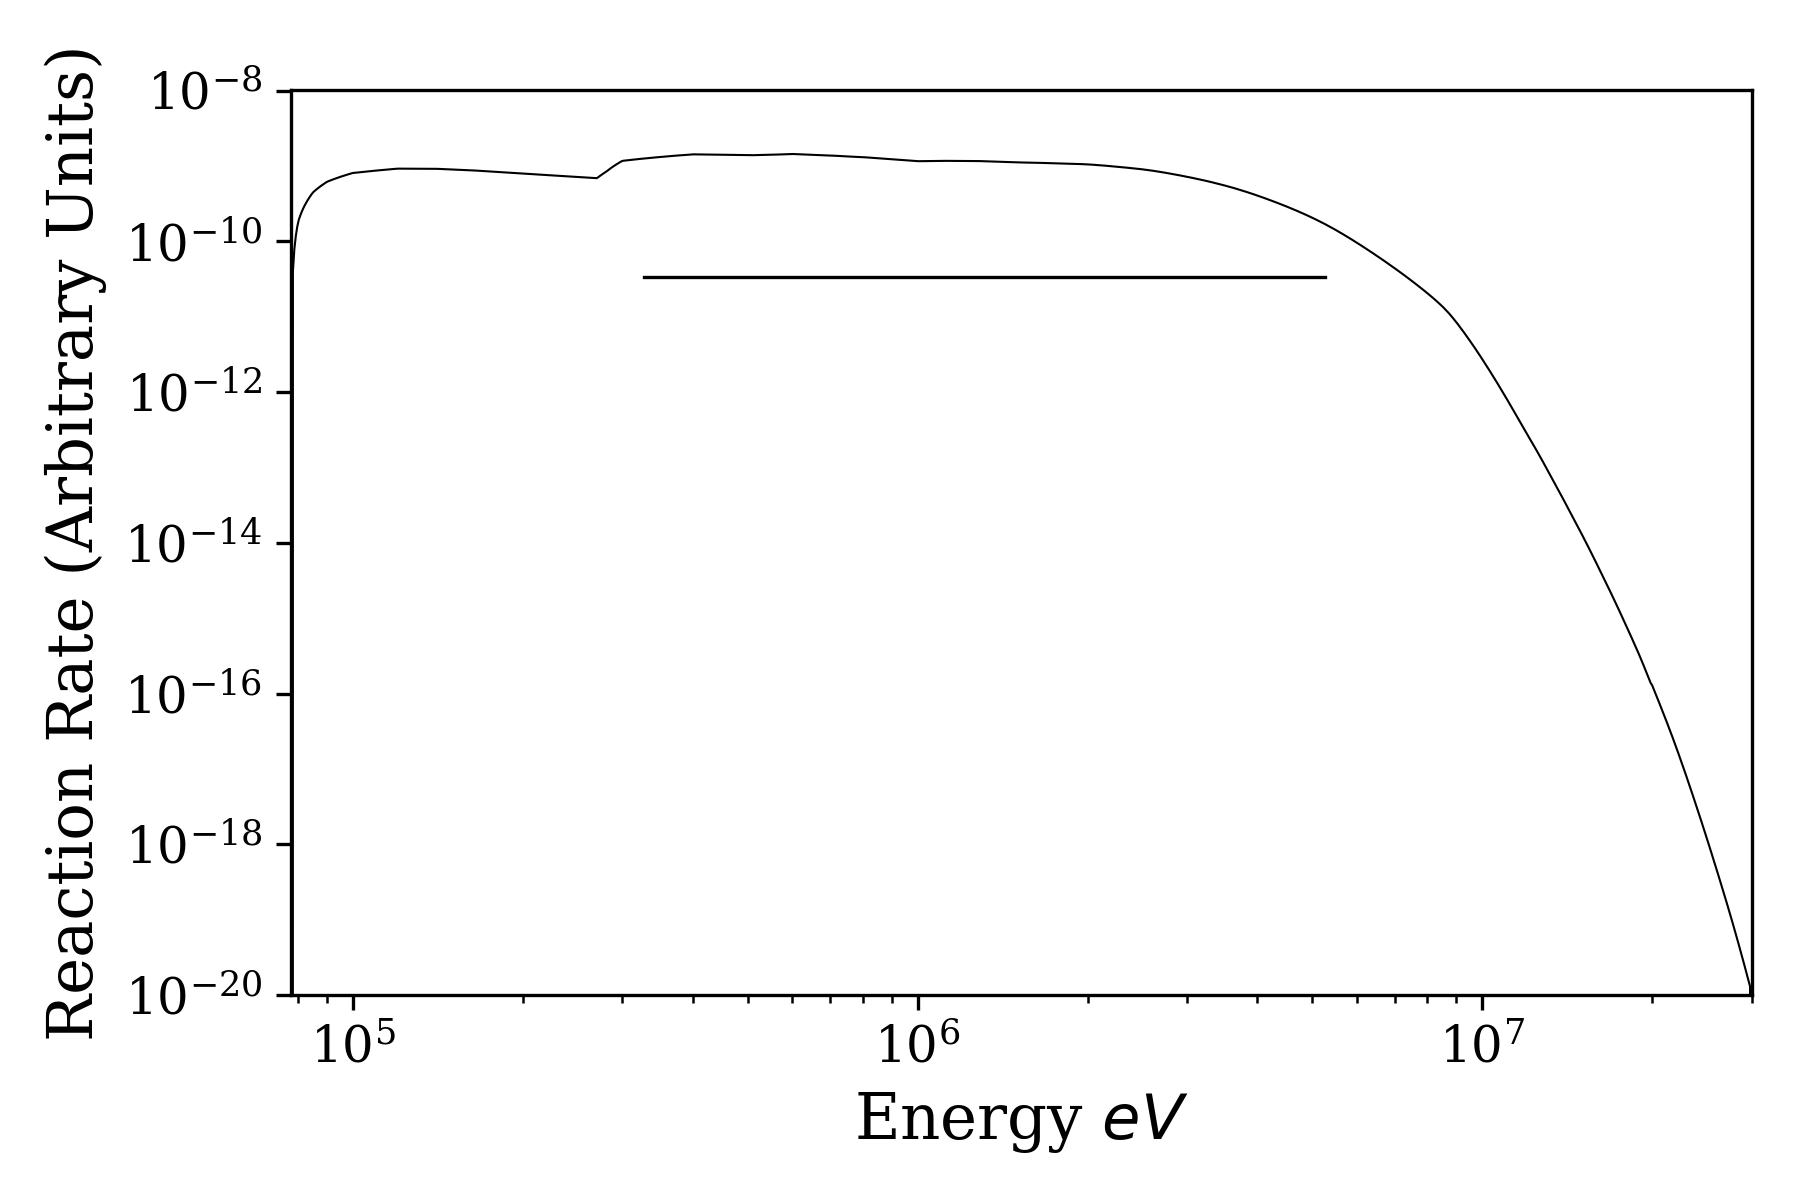
\includegraphics[width=.4\textwidth]{plot/au_n,inelastic_cd}}\\ 

\end{figure}

\begin{table*}[h]
\centering
\begin{tabular}{ |c|c|c|c|c|c|c| }
 \hline
 Reaction & T$_{1/2}$ & ROI (eV) & Important Gammas (keV) \\
 \hline 
 ($n,\gamma$) & 34992000.0 d & 4.08e+00, 7.17e+00 & 412(0.95), 676(0.01), 1088(0.002) \\ 
\hline
 ($n,2n$) & 80092800.0 d & 8.83e+06, 1.35e+07 & 333(0.25), 356(0.94), 426(0.06), 1091(0.002) \\ 
\hline
 ($n,n'$) &  7.8 s & 3.28e+05, 5.28e+06 & 130(0.08), 279(0.75) \\ 
\hline
\end{tabular}
\end{table*}

\newpage

\section*{ Rhodium }

Power Level: 100 kW(th) \\
Time at Power: 600 s \\
Wait Time: 5000 s \\
Total Activity at Removal: 2.20e+05 $\mu Ci$

\begin{table*}[h]
\centering
\begin{tabular}{ |c|c|c|c|c|c|c| }
 \hline
 Position & Mass $mg$ & Start Counting $s$ & Counting Time $s$ & Counting Activity $\mu Ci$ \\
 \hline 
 1 & 0.7 & 5600 & 600 & 7.13e+00\\ 
\hline
 2 & 0.55 & 6200 & 600 & 4.88e+00\\ 
\hline
 3 & 0.5 & 6800 & 600 & 3.91e+00\\ 
\hline
 4 & 0.55 & 7400 & 600 & 3.79e+00\\ 
\hline
\end{tabular}
\end{table*}

\begin{figure}[!ht]
   \centering
   \subfloat[][Position \#1]{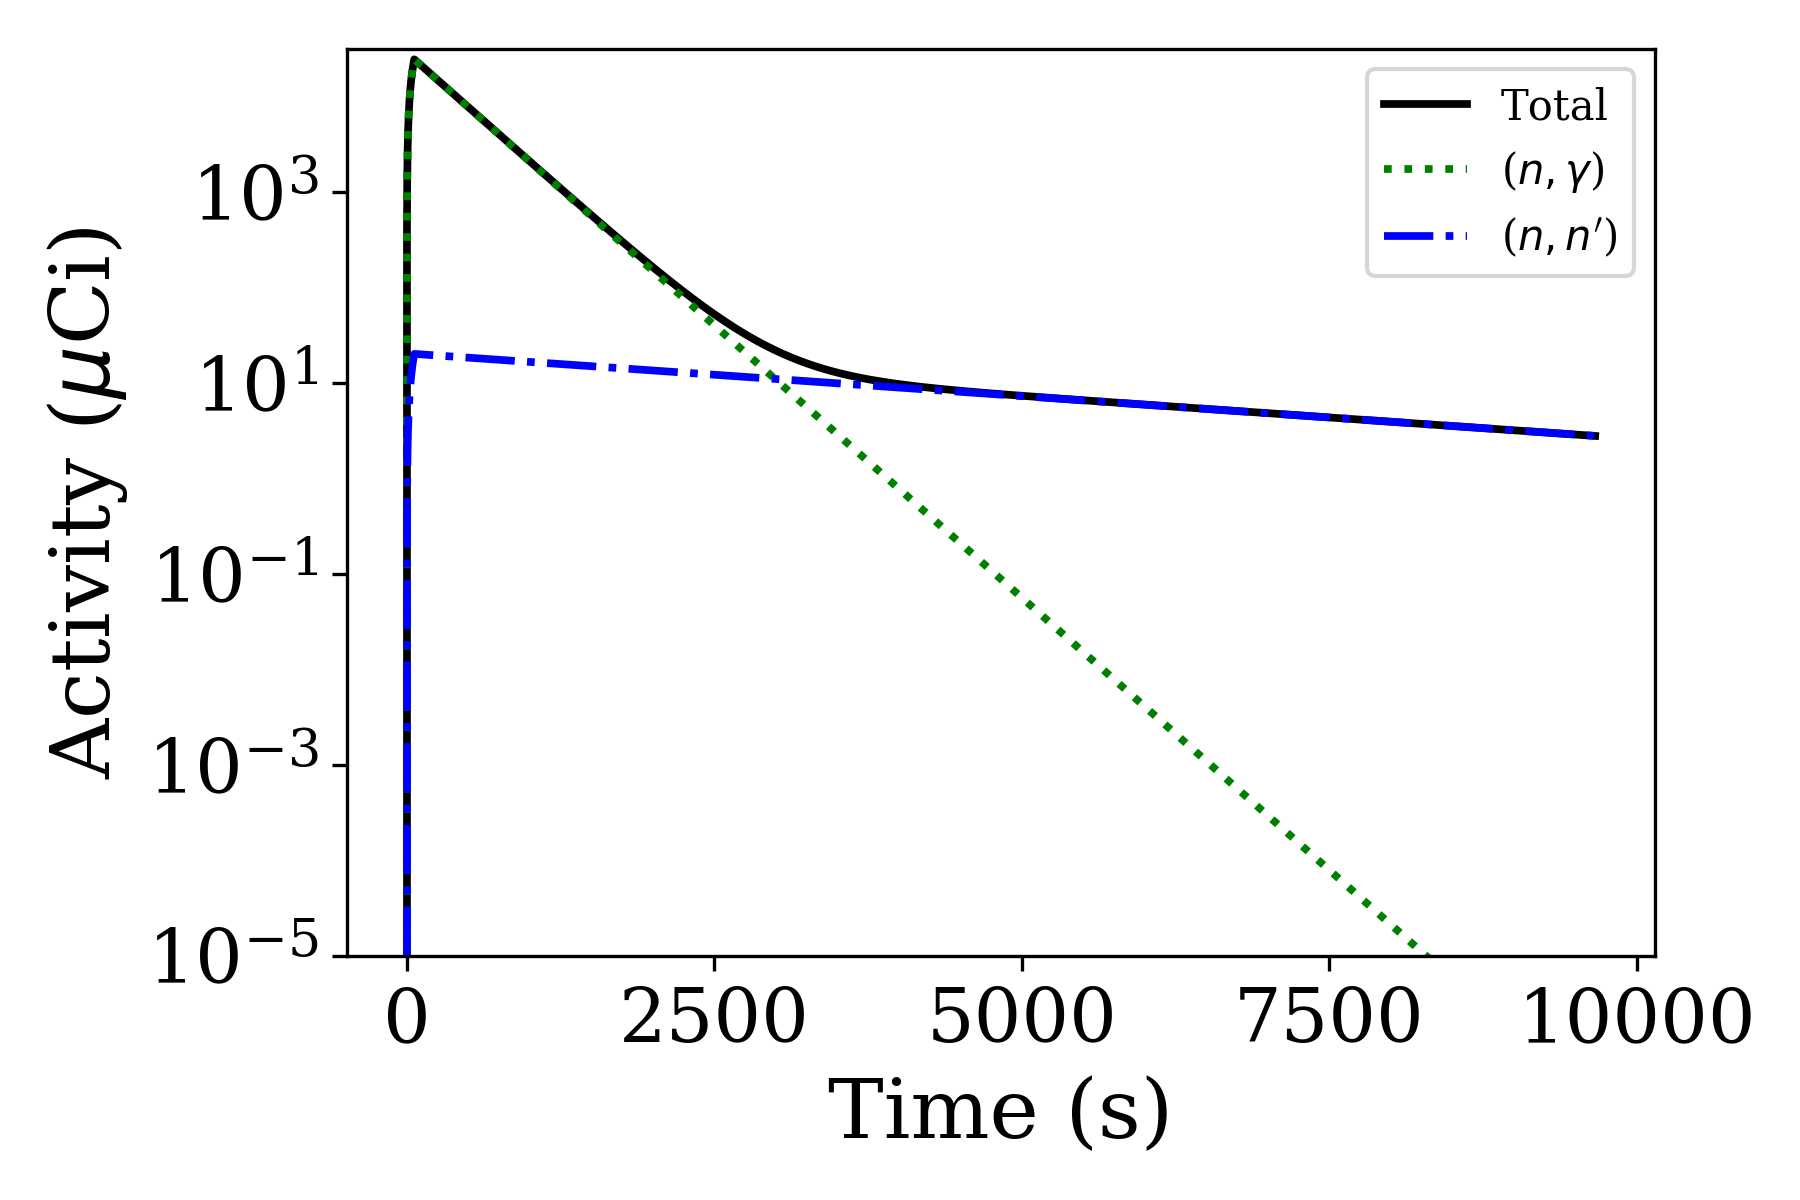
\includegraphics[width=.4\textwidth]{plot/rh1_activity}}\quad
   \subfloat[][ ($n,\gamma$) Reaction Rate]{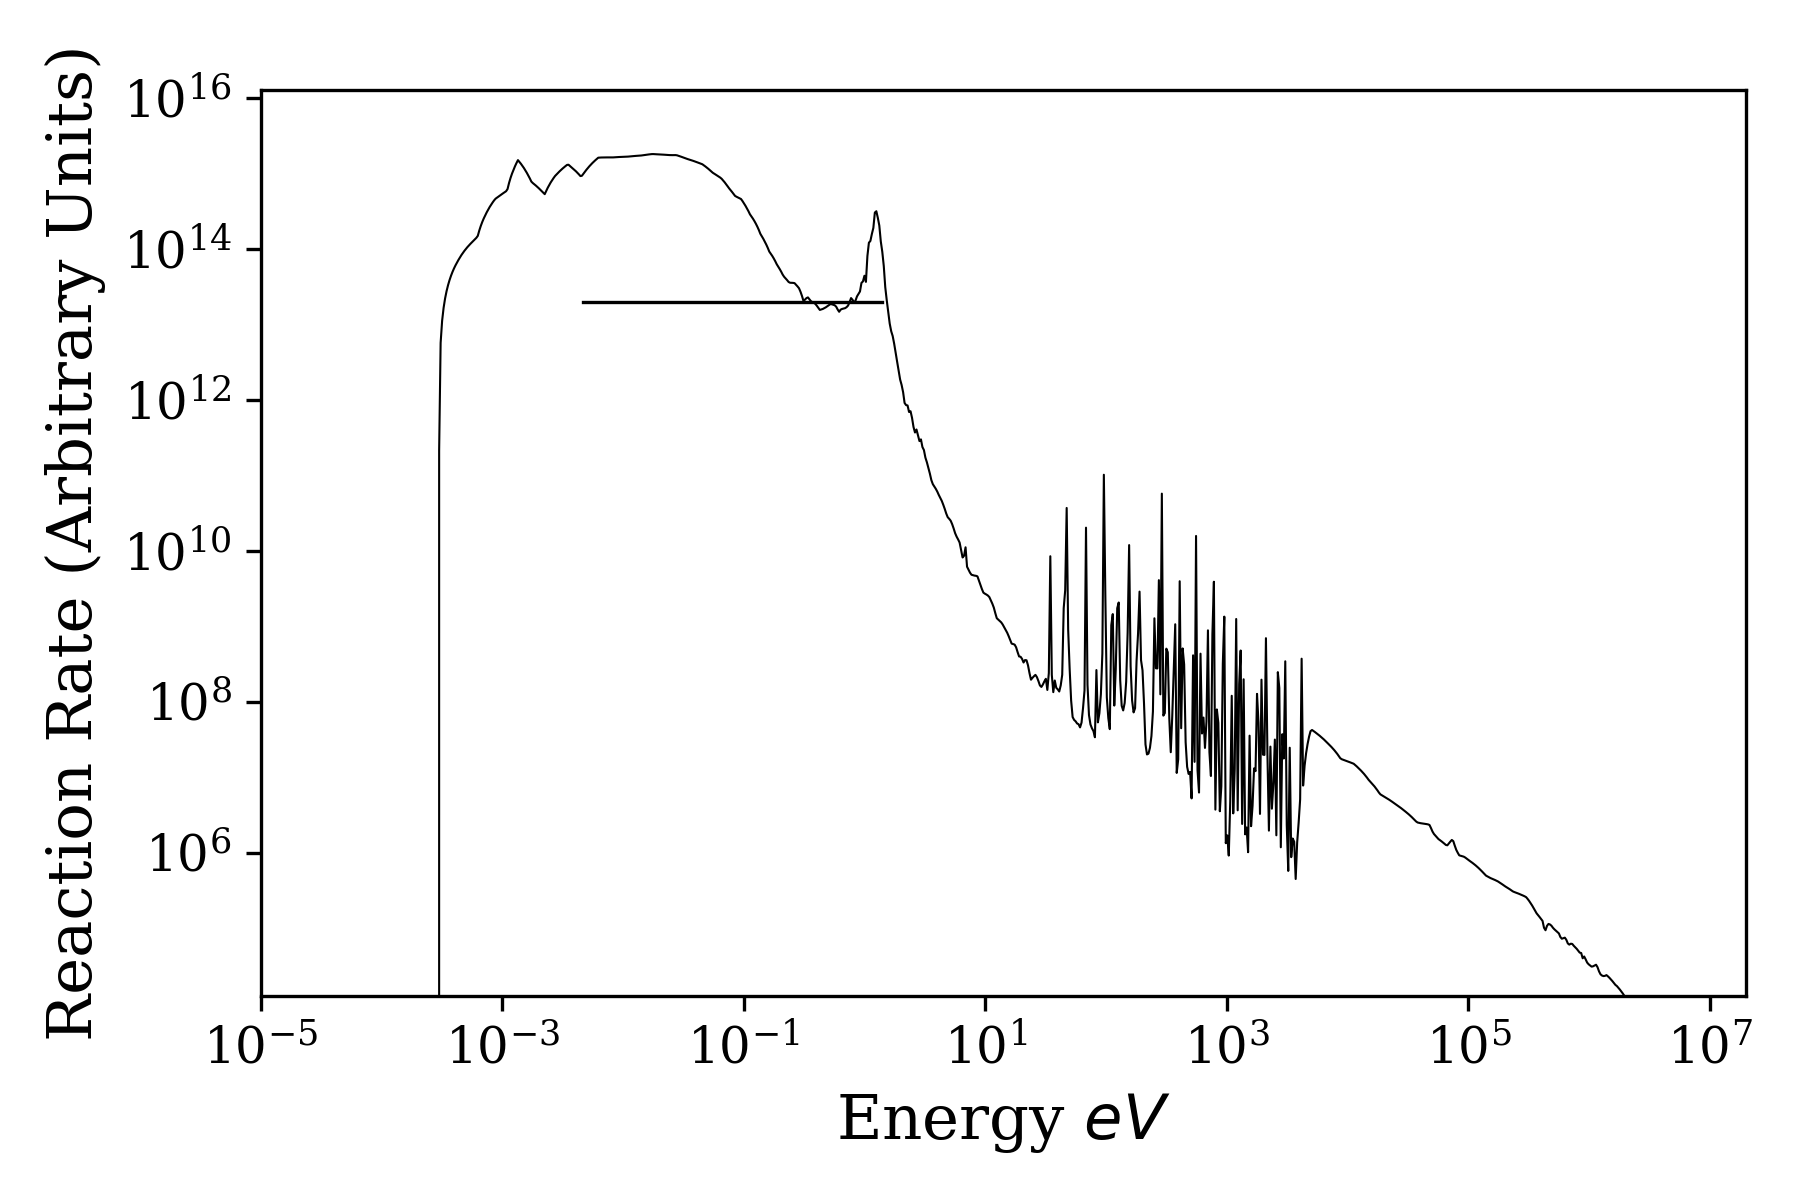
\includegraphics[width=.4\textwidth]{plot/rh_n,gamma}}\\ 
   \subfloat[][ ($n,n'$) Reaction Rate]{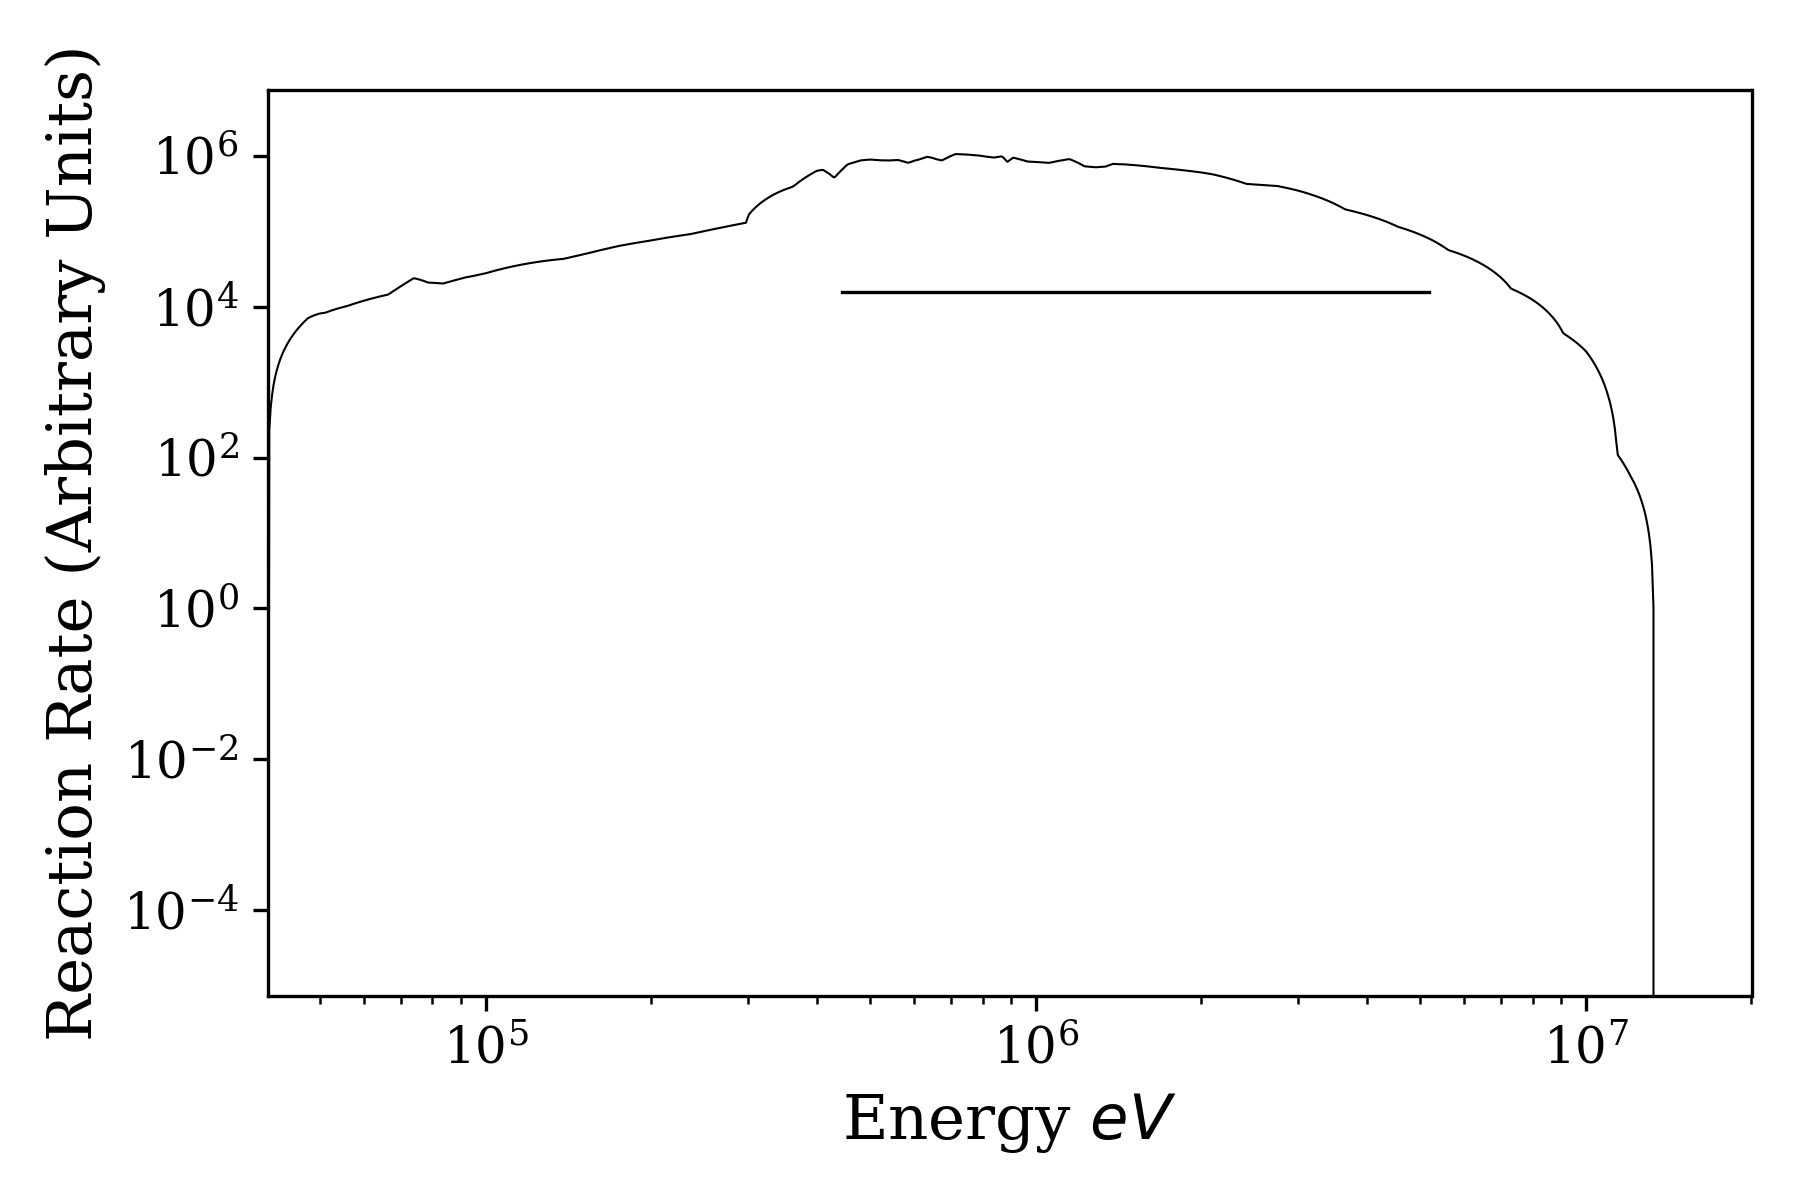
\includegraphics[width=.4\textwidth]{plot/rh_n,inelastic}}\quad 

\end{figure}

\begin{table*}[h]
\centering
\begin{tabular}{ |c|c|c|c|c|c|c| }
 \hline
 Reaction & T$_{1/2}$ & ROI (eV) & Important Gammas (keV) \\
 \hline 
 ($n,\gamma$) &  4.4 m & 4.67e-03, 1.39e+00 & 51(0.47), 78(0.025), 560(0.026), 770(0.0018) \\ 
\hline
 ($n,n'$) & 56.1 m & 4.45e+05, 5.19e+06 & 40(0.004) \\ 
\hline
\end{tabular}
\end{table*}

\newpage

\section*{ Aluminum }

Power Level: 100 kW(th) \\
Time at Power: 3600 s \\
Wait Time: 354870 s \\
Total Activity at Removal: 8.36e+01 $\mu Ci$

\begin{table*}[h]
\centering
\begin{tabular}{ |c|c|c|c|c|c|c| }
 \hline
 Position & Mass $mg$ & Start Counting $s$ & Counting Time $s$ & Counting Activity $\mu Ci$ & Expected Area (Counts) \\
 \hline 
 1 & 0.3 & 358470 & 3600 & 6.27e-05 & 2.79e+02\\ 
\hline
 2 & 0.2 & 362070 & 3600 & 6.09e-05 & 2.72e+02\\ 
\hline
 3 & 0.1 & 365670 & 3600 & 2.25e-05 & 1.00e+02\\ 
\hline
 4 & 0.2 & 369270 & 3600 & 2.00e-05 & 8.91e+01\\ 
\hline
\end{tabular}
\end{table*}

\begin{figure}[!ht]
   \centering
   \subfloat[][Position \#1]{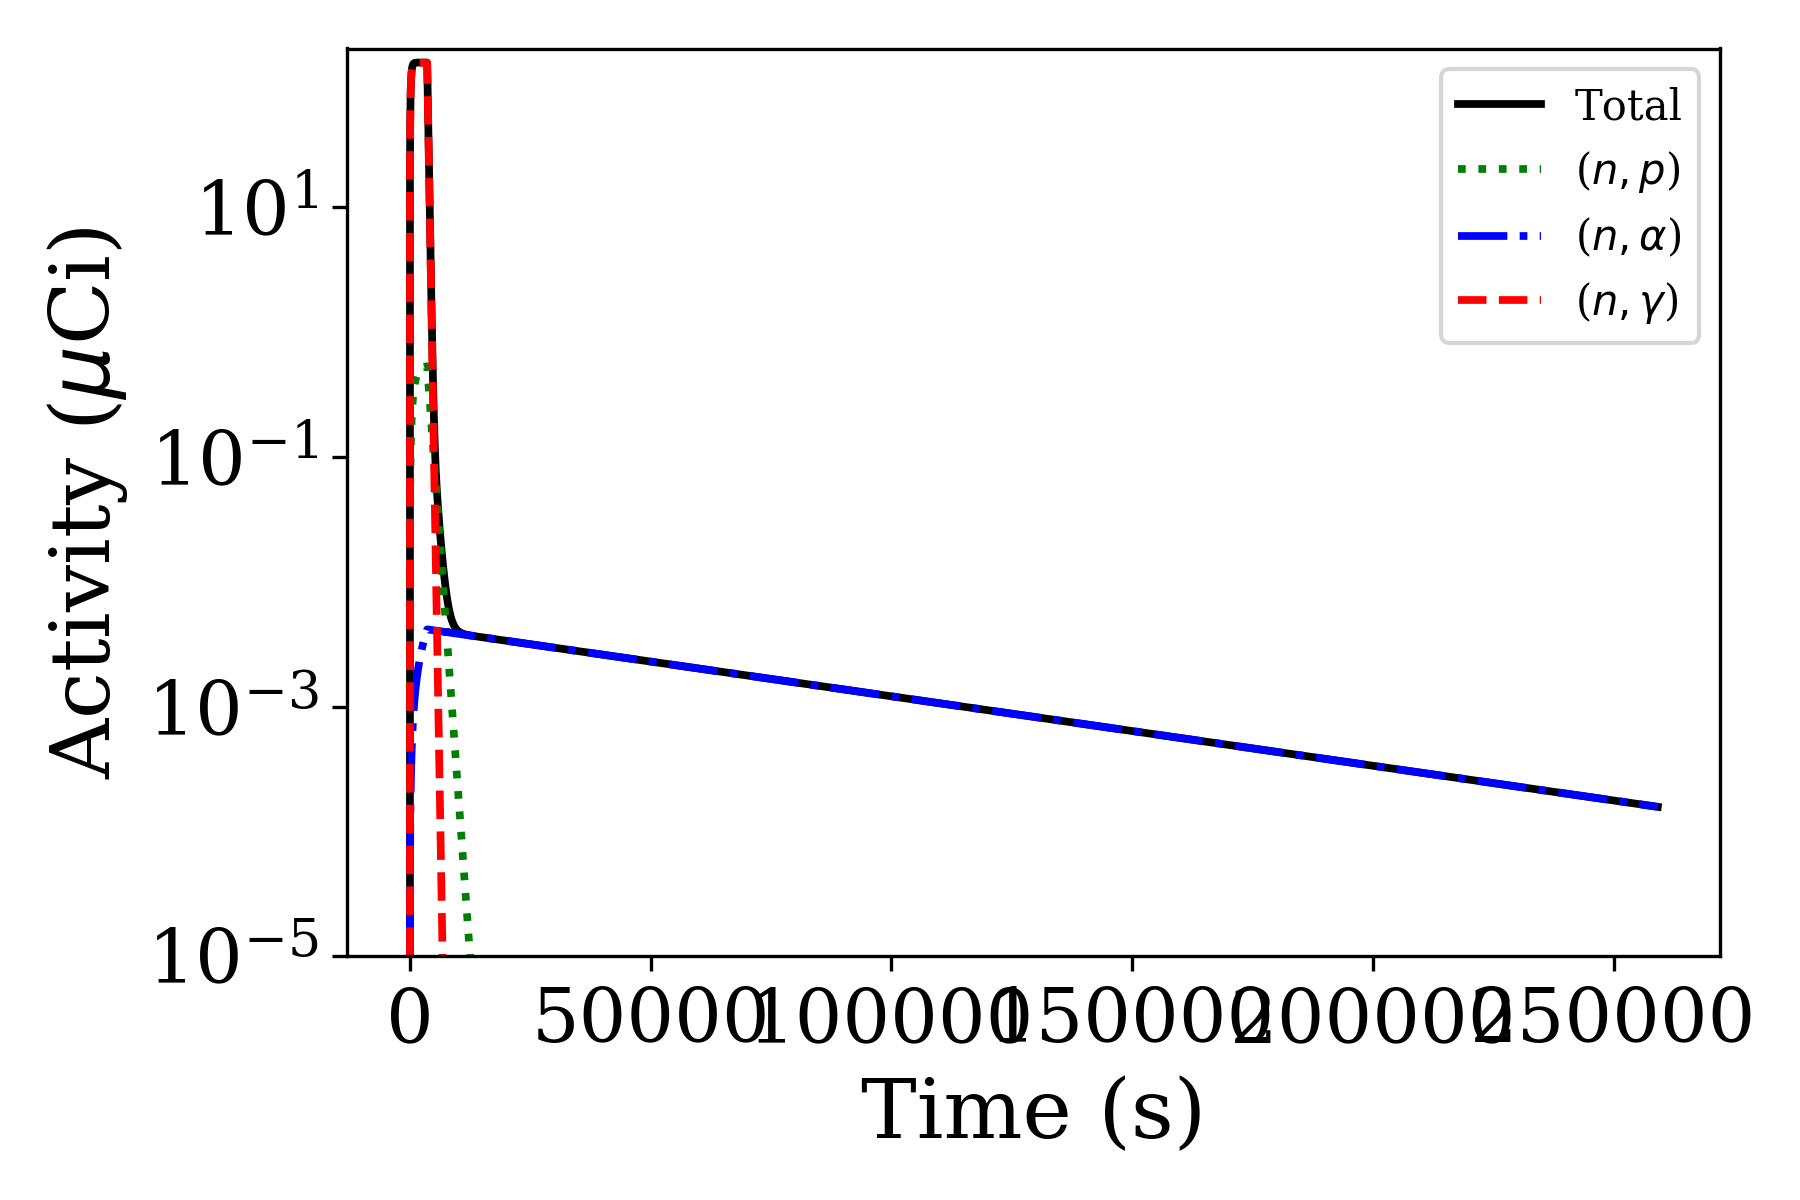
\includegraphics[width=.4\textwidth]{source/plot/al1_activity}}\quad
   \subfloat[][ ($n,p$) Reaction Rate]{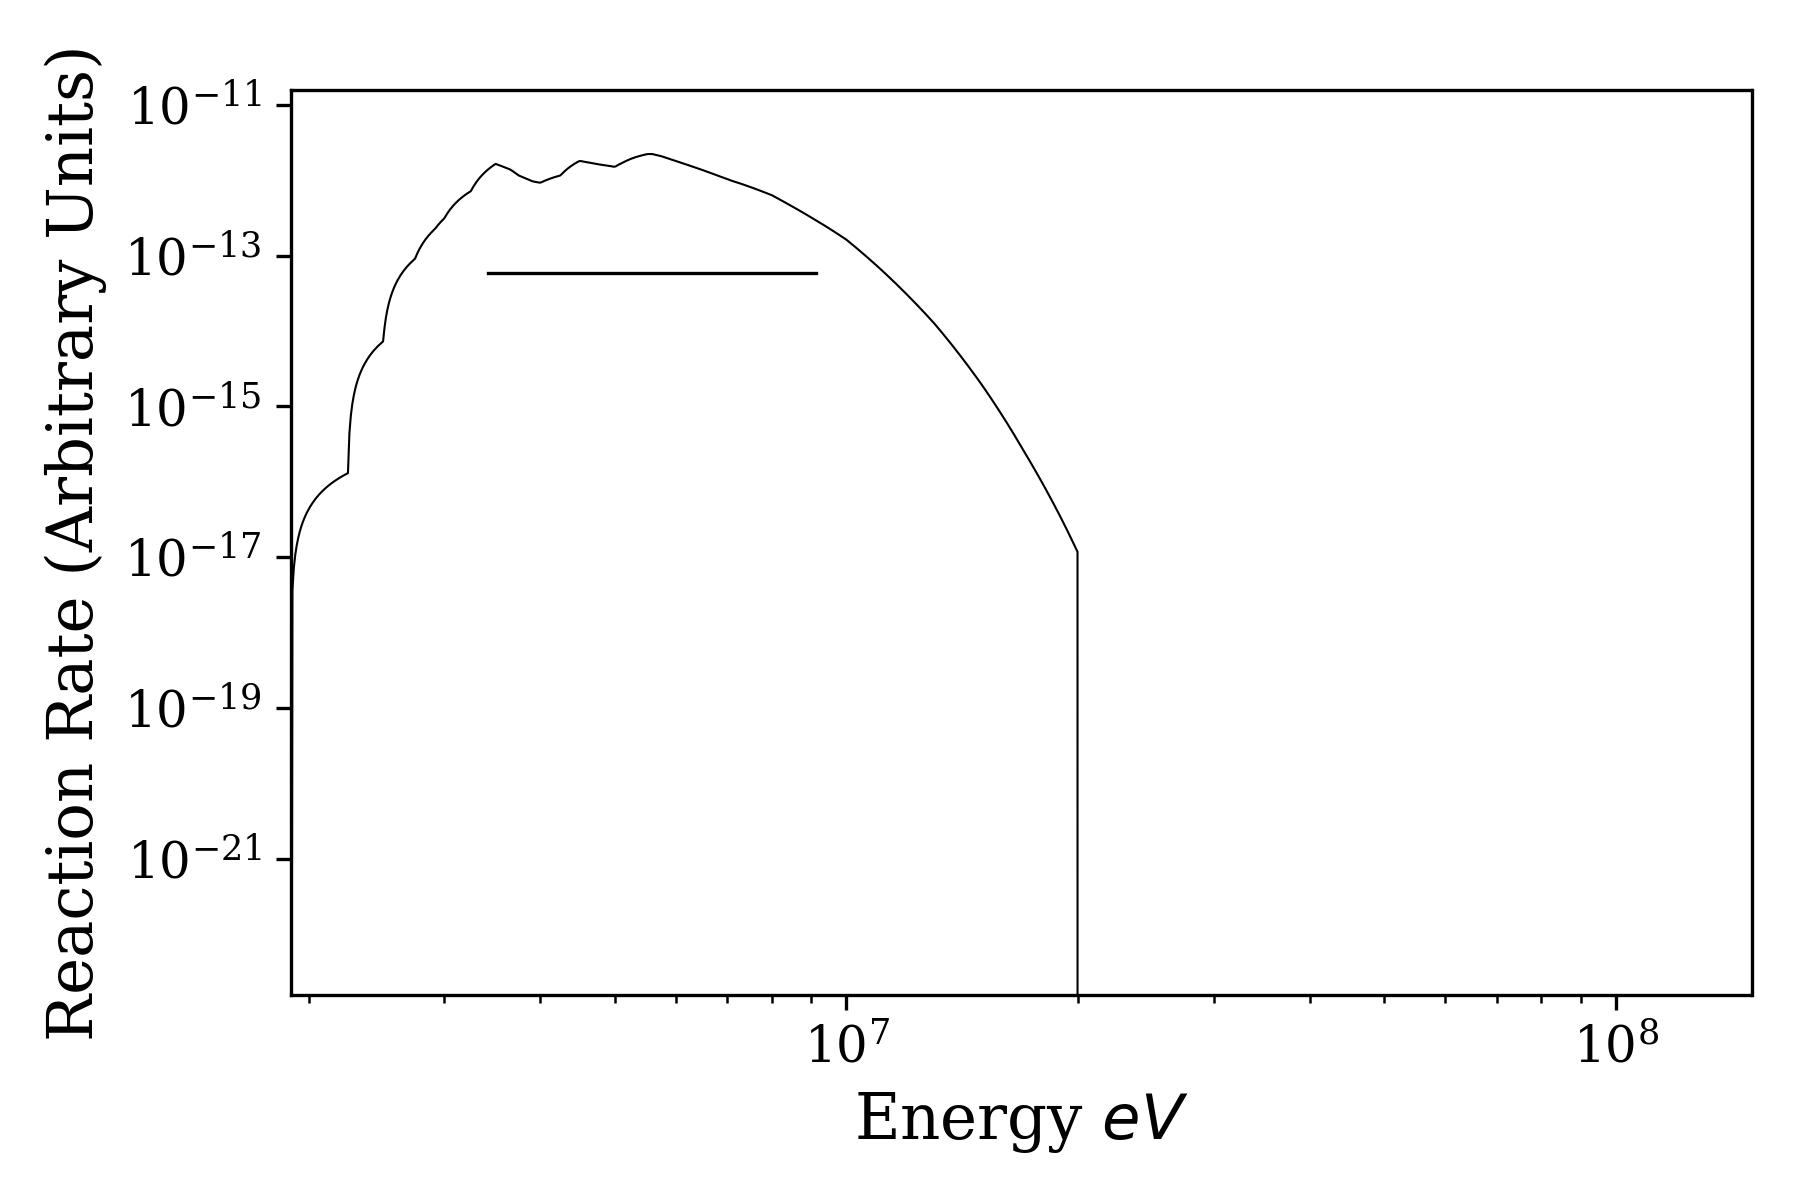
\includegraphics[width=.4\textwidth]{source/plot/al_n,p}}\\ 
   \subfloat[][ ($n,\alpha$) Reaction Rate]{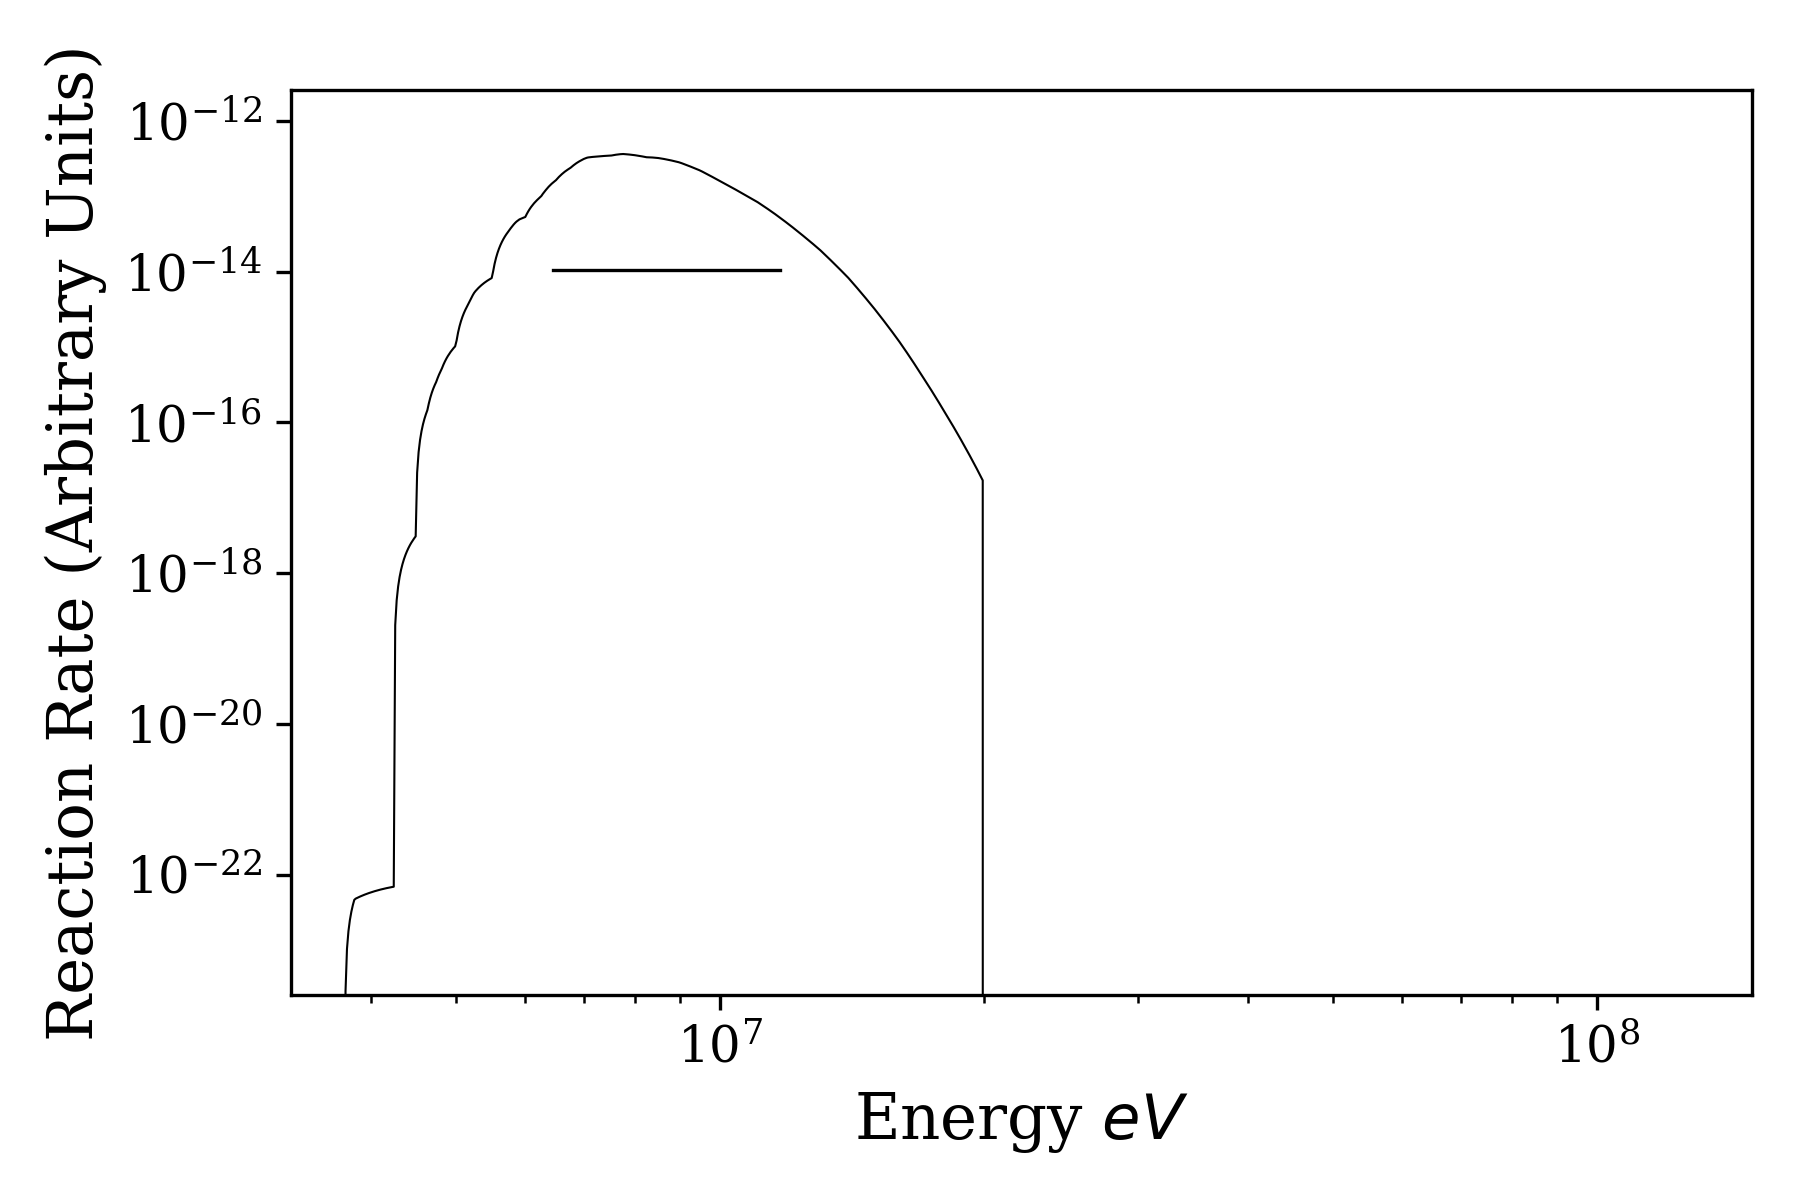
\includegraphics[width=.4\textwidth]{source/plot/al_n,alpha}}\quad 
   \subfloat[][ ($n,\gamma$) Reaction Rate]{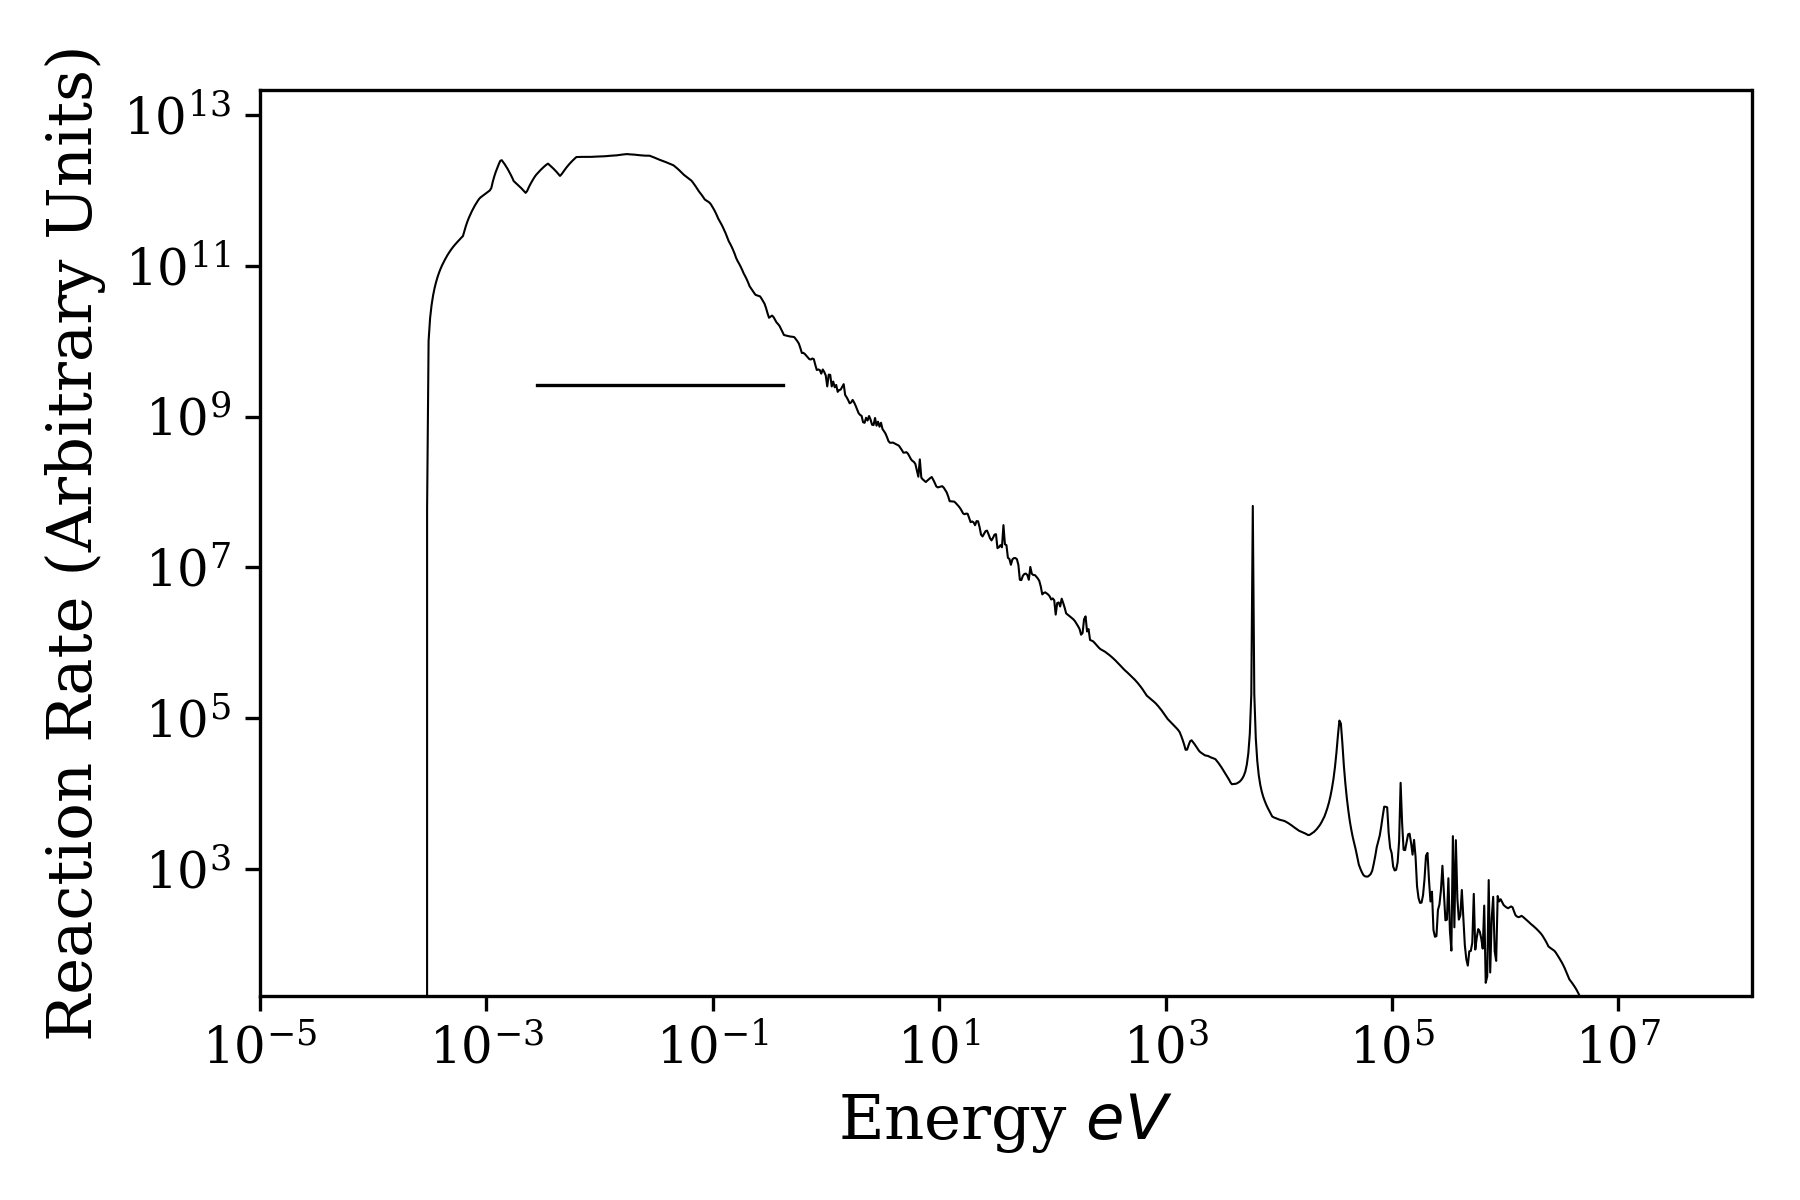
\includegraphics[width=.4\textwidth]{source/plot/al_n,gamma}}\\ 

\end{figure}

\begin{table*}[h]
\centering
\begin{tabular}{ |c|c|c|c|c|c|c| }
 \hline
 Reaction & T$_{1/2}$ & ROI (eV) & Important Gammas (keV) \\
 \hline 
 ($n,p$) &  9.5 m & 3.44e+06, 9.21e+06 & 180(0.007), 840(0.7), 1013(0.3) \\ 
\hline
 ($n,\alpha$) & 15.0 h & 6.48e+06, 1.07e+07 & 1369(1), 2754(1) \\ 
\hline
 ($n,\gamma$) &  2.2 m & 6.67e-03, 4.15e+00 & 1780(1) \\ 
\hline
\end{tabular}
\end{table*}


%%%%%%%%%%%%%%%%%%%%%%%%%%%%%%%%%%%%%%%%%%%%%%%%%%%%%%%%%%%%%
%                       Useful Links
%%%%%%%%%%%%%%%%%%%%%%%%%%%%%%%%%%%%%%%%%%%%%%%%%%%%%%%%%%%%%
\newpage

\section*{Useful Links}

Activation Calculator \\
\href{https://www.ncnr.nist.gov/resources/activation/}{https://www.ncnr.nist.gov/resources/activation/}

\vspace{0.05\textheight}
\noindent
Online Spectrum Catalogs for Ge and Si(Li) \\
\href{http://www4vip.inl.gov/gammaray/catalogs/ge/catalog\_ge.shtml}{http://www4vip.inl.gov/gammaray/catalogs/ge/catalog\_ge.shtml}

\vspace{0.05\textheight}
\noindent
Decay Radiation Search \\
\href{https://www.nndc.bnl.gov/nudat2/indx\_dec.jsp}{https://www.nndc.bnl.gov/nudat2/indx\_dec.jsp}

\vspace{0.05\textheight}
\noindent
Evaluated Nuclear Data File (ENDF) Retrieval \& Plotting \\
\href{https://www.nndc.bnl.gov/sigma/}{https://www.nndc.bnl.gov/sigma/}

% \vspace{0.05\textheight}

% Weighed Foils

% \begin{table*}[h]
% \centering
% \begin{tabular}{ |c|c|c|c|c|c| }
%  \hline
%  Foil ID & Mass ($\mu g$) & Foil ID & Mass ($\mu g$) & Foil ID & Mass ($\mu g$) \\
%  \hline
% uwcd1 &   3.15 & uwcd2 &   3.30 & uwcd3 &   3.30 \\ 
% uwcd4 &   3.30 & rh1 &   0.50 & rh2 &   0.55 \\ 
% rh3 &   0.70 & rh4 &   0.55 & rh5 &   0.70 \\ 
% rh6 &   0.50 & au6 &   5.00 & au7 &   4.30 \\ 
% au8 &   4.35 & au9 &   4.37 & uwau1 &   3.90 \\ 
% uwau2 &   3.45 & uwau3 &   3.40 & uwau4 &   3.30 \\ 
% cd &   0.80 & cd1 &   0.67 & cd2 &   0.75 \\ 
% cd3 &   0.85 & cd4 &   0.95 & cd5 &   0.47 \\ 
% cd6 &  10.90 & cd7 &  11.10 & cd8 &  10.80 \\ 
% cd9 &  11.50 & cd10 &  11.30 & cd11 &  10.40 \\ 
% cd12 &  10.50 & cd13 &  10.50 & cd14 &  10.50 \\ 
% cd15 &  10.70 & cd16 &  10.70 & cd17 &  10.80 \\ 
% cd18 &  10.90 & cd19 &  13.80 & cd20 &  11.00 \\ 
% cd21 &  11.10 & cd22 &  14.00 & cd23 &  10.50 \\ 
% cd24 &  10.80 & cd25 &  10.60 & & \\
%  \hline
% \end{tabular}
% \end{table*}

% \begin{table*}[h]
% \centering
% \caption{Values calculated using NIST online activation calculator found in the useful links section below. Times are estimated to ensure activity below 50 $\mu$Ci and above 2 $\mu$Ci after an hour.}
% \begin{tabular}{ |c|c|c|c|c|c|c| }
%  \hline
%  Reaction & T$_{1/2}$ & E$_{5\%} (eV)$ & E$_{95\%} (eV)$ & P $kW(th)$ & $t_{i}$ (m) & $t_w$ (m) \\
%  \hline
%  Al$^{27}$(n,p)Mg$^{27}$ & 9.458 m & 3.42e+06 & 9.14e+06 & 100 & 4 & 60  \\
%  \hline
%  Al$^{27}$(n,$\alpha$)Na$^{24}$ & 15.03 h & 6.46e+06 & 1.17e+07 & 100 & 4 & 60  \\
%  \hline
%  Rh$^{103}$(n,n')Rh$^{103m}$ & 56.12 m & 0.0 & 0.0 & 1 & 2 & 60  \\
%  \hline
%  In$^{115}$(n,$\gamma$)In$^{116m1}$ & 54 m & 0.0 & 0.0 & 0.001  & 5 & 60  \\
%  \hline
%  In(Cd) & 0.0 & 0.0 & 0.0 & 0.0 & 0.0 & 0.0  \\
%  \hline
%  Au$^{197}$(n,$\gamma$)Au$^{198}$ & 2.7 d & 0.0 & 0.0 & 0.1 & 5 & 60  \\
%  \hline
%  Au(Cd) & 0.0 & 0.0 & 0.0 & 0.0 & 0.0 & 0.0  \\
%  \hline
% \end{tabular}
% \end{table*}

\end{document}
